%sección IV
\section{Método de revisión}\label{sec:metodo-revision}
Con el objetivo de realizar una revisión sistemática de la literatura sobre arquitecturas de seguridad en entornos de computación en la nube, se ha seguido un proceso estructurado basado en las pautas
metodológicas propuestas en~\cite{Runeson2009},~\cite{Kitchenham2010} y~\cite{Petersen2008}.
La aplicación de estas pautas se puede evidenciar en el trabajo de Sepúlveda et al.~\cite{Sepulveda-Rodriguez2021}. De acuerdo con~\cite{Mourao2017} y~\cite{Nguyen2015}, una revisión sistemática de la literatura puede apoyarse en la combinación de
diferentes estrategias de búsqueda con el fin de ampliar la cobertura de estudios relevantes. De esta manera, se usó un enfoque hibrído donde hubo una combinación de búsqueda manual y automatizada. 
Además y con el fin de garantizar la transparencia y reproducibilidad del estudio, se usó la herramienta \textit{SMS-Builder}~\cite{Candela-Uribe2022} que permite realizar la identificación y clasificación de estudios, así como la extracción de datos y la evaluación de calidad de los mismos.
El proceso de revisión sistemática se ha dividido en seis etapas: planeación, búsqueda de estudios, evaluación de calidad, extracción de datos, análisis y clasificación de estudios y resultados. En este contexto, \textit{SMS-Builder} se usó para llevar un registro de las etapas 2, 3, 4 y 5. A continuación, se describen cada una de las etapas del \textbf{SMS} (\textit{Systematic Mapping Study} por su traducción al inglés). Ver Figura~\ref{fig:etapas}.

\begin{figure}[htbp]
    \centering
    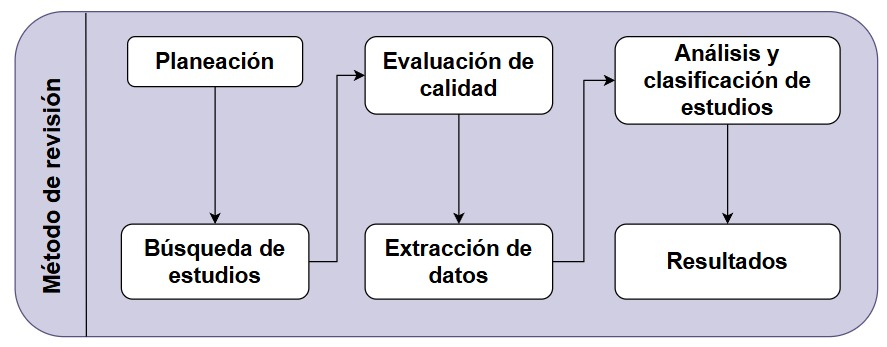
\includegraphics[width=0.5\textwidth]{resources/images/Planeacion/Planeacion.jpeg}
    \caption{Etapas del proceso de construcción de un SMS}\label{fig:etapas}
\end{figure}

% ETAPAS
%subsección 4.1
%Sección 4.1
\subsection{Etapa 1: Planeación}\label{subsec:Planeacion}

En esta etapa, se estableció el propósito general de la investigación y se definieron las metas, así como las preguntas de investigación,
métricas, criterios de clasificación, criterios de inclusión/exclusión y criterios de calidad de los estudios. Ver Figura~\ref{fig:etapa1}.

\begin{figure}[htbp]
        \centering
        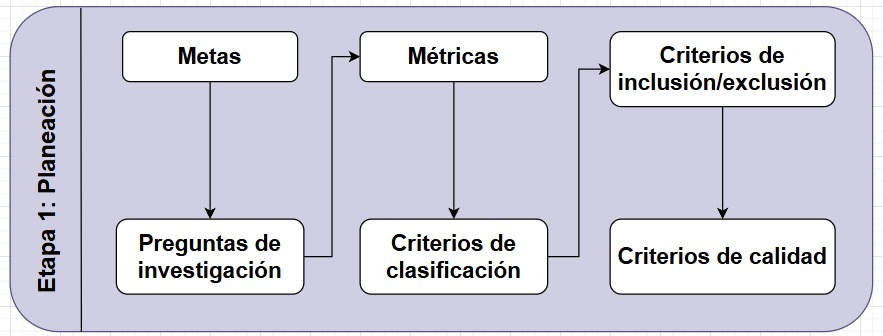
\includegraphics[width=0.5\textwidth]{resources/images/Planeacion/Etapa_1.jpeg}
        \caption{Composición de la etapa de planeación}\label{fig:etapa1}
\end{figure}

\subsubsection{Objetivos}
Teniendo en cuenta los aspectos descritos en la sección de motivación~\ref{sec:Motivacion}, se definieron 2 metas generales para la 
revisión sistemática de la literatura que se presentan en el cuadro~\ref{tab:metas}.

\begin{table}[htbp]
    \centering
    \begin{tabular}{>{\centering\arraybackslash}m{0.5cm}>{\arraybackslash}m{7cm}}
        \hline
        \textbf{Metas} & \textbf{Descripción} \\
        \hline\\
        M1 & Identificar trabajos relacionados con la seguridad de la información en entornos de computación en la nube, según su enfoque, mecanismos de protección, gestión de riesgos y examinando su grado de alineación con estándares internacionales de referencia, tales como las normas ISO/IEC 27001, 27017 y 27018, en contextos institucionales de investigación. \\
        \\
        M2 & Determinar una estructura de clasificación de trabajos que aborden la seguridad de la información en la computación en la nube como soporte para las funciones universitarias de investigación, docencia y gestión institucional. \\\\
        \hline
        \vspace{1pt}
    \end{tabular}
    \caption{Metas del estudio}\label{tab:metas}
\end{table}

\subsubsection{Pregunta de investigación}
Para la construcción de las preguntas de investigación (RQ, por sus siglas en inglés) se utilizó GQM \textit{(Goal Question Metric)}~\cite{Needleman2002} y el modelo PICOC~\cite{petticrew2008systematic}.
Este modelo permite establecer aspectos como ``Población'', ``Intervención'', ``Comparación'', ``Salida'' y ``Contexto'' que sirven para situar el trabajo a realizar.
Ver cuadro~\ref{tab:PICOC}.


\begin{table}[tbp]
    \scriptsize % reduce tamaño del texto
    \centering
    \renewcommand{\arraystretch}{1.0}
    \begin{tabularx}{\columnwidth}{>{\centering\arraybackslash}m{0.18\columnwidth} >{\raggedright\arraybackslash}X}
        \hline
        \textbf{Aspecto} & \textbf{Descripción} \\
        \hline
        Población & Estudios relacionados a las buenas prácticas, normativas, controles y marcos de referencias internacionales para la seguridad de la computación en la nube. \\
        Intervención &
        1. Identificación de un conjunto de buenas prácticas, controles, metodologías, herramientas y tecnologías.~\newline
        2. Identificar el modelo taxonómico de los trabajos. \\
        Comparación &
        1. Estudios que han hecho uso de normas internacionales para la seguridad de la información de la computación de la nube y que se demuestre mayor tasa de éxito en contrarrestar ataques informáticos.~\newline
        2. Se examina la importancia de la ciberseguridad y su impacto en trabajos de docencia, investigación y la gestión institucional.~\newline
        3. Se aplican criterios de inclusión y exclusión. \\
        Salida & Documentos y estructura de clasificación sobre arquitecturas de seguridad relacionados con las normativas internacionales que han impactado en proyectos de docencia, investigación y gestión institucional. \\
        Contexto & Gestión institucional, seguridad de la computación en la nube, confidencialidad, integridad y disponibilidad de servicios en la nube. \\
        \hline
        \vspace{1pt}
    \end{tabularx}
    \caption{Aspectos del modelo PICOC}\label{tab:PICOC}
\end{table}

Teniendo en cuenta la información del modelo PICOC, se definieron 2 RQ.\@ Ver cuadro~\ref{tab:preguntas}.

\begin{table*}[!t]
    \centering
    \renewcommand{\arraystretch}{1.4}
    \begin{tabularx}{\textwidth}{>{\centering\arraybackslash}m{0.02\textwidth} >{\centering\arraybackslash}m{0.04\textwidth} >{\raggedright\arraybackslash}X >{\raggedright\arraybackslash}X}
    \toprule
    \textbf{Meta} & \textbf{Pregunta} & \textbf{Descripción} & \textbf{Motivación} \\
    \midrule
    G1 & Q1 & ¿Qué trabajos abordan arquitecturas de seguridad en entornos de computación en la nube para contextos institucionales y universitarios, y qué enfoques de protección de activos, gestión de riesgos y controles de seguridad proponen, en relación con estándares y buenas prácticas internacionales? & Sobre las arquitecturas de seguridad en entornos de computación en la nube, alineadas con los controles de las normas ISO/IEC 27001, 27017 y 27018 y demás estándares internacionales y su impacto en contextos institucionales y universitarios: \newline
    1. Reconocer cómo las arquitecturas de seguridad en la nube apoyan la protección de la información en procesos de investigación, docencia y gestión académica.~\newline
    2. Identificar los mecanismos, controles y componentes de seguridad utilizados en las arquitecturas analizadas.~\newline
    3. Determinar el contexto y propósito de aplicación de las arquitecturas consideradas. \\
    \midrule
    G2 & Q2 & ¿Cuál es la estructura taxonómica de las arquitecturas de seguridad en la computación en la nube que contribuyen al fortalecimiento de funciones institucionales en entornos universitarios, tales como la investigación, la docencia y la gestión institucional? & Sobre las arquitecturas de seguridad en la computación en la nube aplicadas a entornos universitarios y su contribución al fortalecimiento de funciones institucionales: \newline
    1. Reconocer cómo se clasifican las arquitecturas de seguridad propuestas en la literatura para la protección de activos de información en la nube.~\newline
    2. Identificar el aporte de los controles de seguridad y mecanismos implementados en las arquitecturas evaluadas.~\newline
    3. Determinar el impacto de estas arquitecturas en la mejora de la gestión tecnológica y administrativa dentro de instituciones de educación superior. \\
    \bottomrule
    \vspace{1pt}
    \end{tabularx}
    \caption{Preguntas de investigación y su motivación}\label{tab:preguntas}
\end{table*}

\subsubsection{Métricas}

Se establecieron las métricas del estudio mediante un enfoque cuantitativo, conforme a la estructura de clasificación. Los detalles de 
dichas métricas se presentan en el cuadro~\ref{tab:metricas}. Los criterios definidos limitaron la validez de los documentos a un periodo 
de tres años, con el fin de favorecer la actualidad del estudio. Asimismo, el tipo de fuente se restringió a estudios primarios, con el 
propósito de asegurar un mayor rigor en la revisión por pares.

\begin{table}[htbp]
    \centering
    \renewcommand{\arraystretch}{1.3}
    \begin{tabularx}{\columnwidth}{>{\centering\arraybackslash}m{0.06\textwidth} >{\raggedright\arraybackslash}X}
    \toprule
    \textbf{Métrica} & \textbf{Descripción} \\
    \midrule
    M1 & Cantidad de trabajos referentes a  metodologías, marcos de referencia y buenas prácticas  de la seguridad de la computación en la nube. \\
    M2 & Cantidad de trabajos con referentes de herramientas tecnológicas y tecnologías relacionados con la seguridad de la computación en la nube. \\
    M3 & Cantidad de trabajos relacionados con casos de estudio referentes a la seguridad de la computación en la nube. \\
    M4 & Cantidad de trabajos referentes al fortalecimiento de la seguridad en la computación en la nube en funciones institucionales de entornos universitarios. \\
    \bottomrule
    \vspace{1pt}
    \end{tabularx}
    \caption{Métricas definidas para el análisis}\label{tab:metricas}
\end{table}

\subsubsection{Tópicos de investigación}

Las preguntas de investigación y el modelo PICOC sirven como línea base para definir los tópicos considerados relevantes en el estudio.
Los tópicos definidos para cada pregunta fueron los siguientes:

\begin{itemize}
    \item \textbf{Q1:} \textit{Security}, \textit{ISO/IEC 27001}, \textit{Architecture}, \textit{Security Controls}, \textit{Cloud Computing}, \textit{Cybersecurity}, \textit{SECURITY INFORMATION AND EVENT MANAGEMENT (SIEM)}.

    \item \textbf{Q2:} \textit{Classification}, \textit{Architecture}, \textit{Taxonomy}, \textit{Cloud Computing}, \textit{Security}, \textit{ZERO-TRUST}.
\end{itemize}

La definición de los tópicos de investigación se realizó considerando los dominios conceptuales más relevantes asociados a cada pregunta de investigación.\\

\subsubsection{Criterios de inclusión y exclusión}
\mbox{}\\
\begin{table*}[!t]
    \centering
    \renewcommand{\arraystretch}{1.0}
    \begin{tabularx}{\textwidth}{>{\centering\arraybackslash}m{0.15\textwidth} >{\raggedright\arraybackslash}X >{\raggedright\arraybackslash}X}
    \toprule
    \textbf{Categoría} & \textbf{Inclusión} & \textbf{Exclusión} \\
    \midrule
    Campos & Resumen, titulo y palabras clave & --- \\
    \midrule
    Tipo de publicación & Artículos y capitulos publicados en revistas científicas o académicas y actas de congresos & Informe técnico, actas de congresos y tesis. \\
    \midrule
    Área/Disciplina & Administración, Informática, Tecnologías de la Información y Ciberseguridad. & Áreas no relacionadas con la gestión, Informática, Tecnologías de la Información y Ciberseguridad. \\
    \midrule
    Período & Entre 2020 to 2026 & Menos de 2020 \\
    \midrule
    Idioma & Inglés & --- \\
    \bottomrule
    \vspace{1pt}
    \end{tabularx}
    \caption{Criterios de inclusión y exclusión}\label{tab:criterios}
\end{table*}
Los criterios de inclusión y exclusión se definieron con el fin de garantizar que los estudios seleccionados fueran pertinentes para 
responder a las preguntas de investigación y cumplir con los objetivos del estudio. Dichos criterios se presentan en la Tabla~\ref{tab:criterios}.
En primer lugar, se consideraron únicamente los campos de título, resumen y palabras clave para la identificación inicial de los estudios. 
En cuanto al tipo de publicación, se incluyeron artículos y capítulos publicados en revistas científicas, académicas y en actas de 
congresos, mientras que se excluyeron informes técnicos y tesis. Respecto al área o disciplina, se incluyeron estudios pertenecientes a 
los campos de Administración, Informática, Tecnologías de la Información y Ciberseguridad, excluyendo aquellos que no estuvieran 
relacionados con estas áreas. Asimismo, se estableció un período de publicación comprendido entre los años 2020 y 2026, con el objetivo de 
priorizar estudios recientes y reflejar el estado actual de la investigación en el área. Finalmente, se consideraron únicamente estudios 
escritos en inglés, con el propósito de asegurar la accesibilidad y comparabilidad de la literatura analizada.

\subsubsection{Criterios de calidad}\label{subsec:criterios_calidad}

Para finalizar la etapa de planeación, se definieron tres criterios de calidad. \\

El primer criterio de calidad es una adaptación del CVI \textit{(Content Value Index)}.
En este caso, los artículos se evaluaron para determinar si cumplen con los criterios de inclusión y exclusión definidos y si son relevantes
para las preguntas de investigación. Se usó una escala cuantitativa de 0 a 5, donde 0 indica una baja relación con las metas del SMS y 5 
indica una alta relación. Ver formula~\ref{eq:cvi}. En esta formula, \textbf{K} es el número impar de evaluadores y \textbf{\textit{f (n)}} 
es la frecuencia de respuestas para cada valor de la escala.\\

\begin{equation}
    \label{eq:cvi}
    CVI = \frac{\sum_{n=1}^{k} f(n)}{k}
\end{equation}

El segundo criterio de calidad es el número de citas de cada estudio de acuerdo con la fecha de publicación (\textbf{A}), el cual se 
denomina SCI \textit{(Scientific Citation Index)}. Ver formula~\ref{eq:sci}. En esta formula, \textbf{C} es el número de citas entre 2022 y 
2024 y \textbf{A} es el tiempo de publicación del estudio. Así, un artículo publicado en 2024 con las misma cantidad de citas que un 
artículo publicado en 2022 tendrá un SCI más alto.\\

\begin{equation}
    \label{eq:sci}
    SCI = \frac{C}{A}
\end{equation}

El tercer criterio de calidad corresponde a la relación de los estudios con las preguntas de investigación. Este criterio se denomina 
IRRQ \textit{(Index of Relationship to Research Questions)}. Ver formula~\ref{eq:irrq}.

\begin{equation}
    \label{eq:irrq}
    IRRQ = \frac{N}{2}
\end{equation}

\textbf{N} corresponde al número de preguntas de investigación que el estudio responde. Este valor se divide en 2 porque es el número de 
preguntas de investigación definidas en la etapa de planeación.\\

%subsección 4.2
%% Definición de variables
\newcommand{\totalStudies}{181}
\newcommand{\databaseStudies}{166}
\newcommand{\snowballStudies}{15}
%Que yo recuerde en nuestro trabajo aún no hicimos inclusión directa de trabajos, sin embargo lo coloco aquí para el futuro.
\newcommand{\directInclusionStudies}{0}


% subseccion 4.2 ------- BUSQUEDA DE ESTUDIOS.
\subsection{Etapa 2: Búsqueda de Estudios}

Esta etapa presentan las estrategias de búsqueda utilizadas en el SMS\@. Estas estrategias serán definidas y descritas en detalle en las subsecciones~\ref{subsubsec:busqueda-bases-datos} hasta~\ref{subsubsec:resultados-busqueda}. Ver Figura~\ref{fig:busqueda-estudios}.
El resultado de esta etapa fueron \totalStudies{} estudios obtenidos. De los cuales hubo \databaseStudies{} estudios por bases de datos y  \snowballStudies{} estudios por bola de nieve.


% -------- Tabla : Actividades de la etapa de búsqueda de estudios. ------------
\begin{figure}[htbp]
	\centering
	\vspace{10pt}
	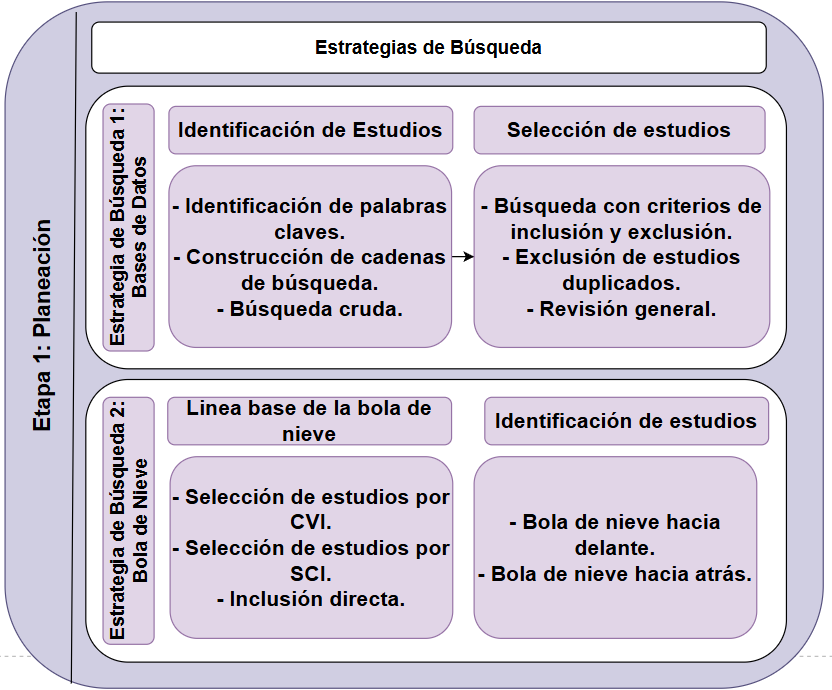
\includegraphics[scale=0.33]{resources/images/Planeacion/Estrategias_busqueda.png}
		\caption{Actividades de la etapa de búsqueda de estudios.}\label{fig:busqueda-estudios}
\end{figure}

\subsubsection{Definiendo la Estrategia de Búsqueda}

Para desarrollar este SMS, se ha implementado una metodología híbrida. Esta metodología tiene como objetivo conseguir una cantidad más amplia de estudios indexados y procedentes de múltiples fuentes, superando los resultados que ofrecen en las bases de datos. De esta manera, integramos dos técnicas de búsqueda. La técnica inicial se denomina ``Búsqueda en bases de datos'' la cual consiste en realizar una búsqueda automatizada dentro de bases de datos académicas indexadas~\cite{Jalai-01}. La técnica secundaria recibe el nombre de \textit{Snowballing} o bola de nieve y representa un procedimiento manual fundamentado en una previa recolección de textos iniciales para identificar investigaciones adicionales mediante sus bibliografías y citaciones~\cite{Jalai-01,Goodman-01}.
Para apoyar el proceso llevado a cabo en este SMS, hemos utilizado los siguientes elementos: Bases de datos académicas, El software SMS-Builder desarrollado por~\cite{Candela2022100935} diseñado específicamente para facilitar la construcción de estudios de mapeo sistemático, Herramientas para apoyar la gestión de referencias como Mendeley y la busqueda de las mismas como Google Scholar.


%sub-subseccion 4.2.1 ----- BUSQUEDA POR BASES DE DATOS 
%sub-subseccion 4.2.1 
\subsubsection{Estrategia de Búsqueda 1: Bases de Datos}\label{subsubsec:busqueda-bases-datos}

%%% Variables de frecuencia por cada base de datos. 
\newcommand{\wos}{933}
\newcommand{\ieee}{3022}
\newcommand{\spr}{35788}
\newcommand{\tf}{761}
\newcommand{\sd}{2539}
\newcommand{\tot}{43043}
%%% Variables de contrubución porcetual
\newcommand{\wosp}{\fpeval{round (\wos*100/\tot,2)}}
\newcommand{\ieeep}{\fpeval{round (\ieee*100/\tot,2)}}
\newcommand{\sprp}{\fpeval{round (\spr*100/\tot,2)}}
\newcommand{\tfp}{\fpeval{round (\tf*100/\tot,2)}}
\newcommand{\sdp}{\fpeval{round (\sd*100/\tot,2)}}

%%%%% ------------------------------------------------

%%% Variables de frecuencia por cada base de datos. 
\newcommand{\iwos}{10}
\newcommand{\iieee}{124}
\newcommand{\ispr}{947}
\newcommand{\itf}{37}
\newcommand{\isd}{142}
\newcommand{\itot}{1260}
%%% Variables de contribución porcentual
\newcommand{\iwosp}{\fpeval{round (\iwos*100/\itot,2)}}
\newcommand{\iieeep}{\fpeval{round (\iieee*100/\itot,2)}}
\newcommand{\isprp}{\fpeval{round (\ispr*100/\itot,2)}}
\newcommand{\itfp}{\fpeval{round (\itf*100/\itot,2)}}
\newcommand{\isdp}{\fpeval{round (\isd*100/\itot,2)}}

%Cantidad de estudios excluídos por ser duplicados
\newcommand{\numEstEx}{3}

%Cantidad de estudios luego de depuración = (estudios totales luego de exclusión - estudios duplicados)
%1257
\newcommand{\depTot}{\fpeval{\itot-\numEstEx}}

%Cantidad de estudios depurados por el screening
\newcommand{\screen}{1091}

%Cantidad de estudios totales luego del screening
%166
\newcommand{\screenTot}{\fpeval{\depTot-\screen}}

Esta estrategia comprende dos componentes. El primer componente se denomina ``Identificación de estudios''. Se enfoca en establecer las 
palabras clave para construir las cadenas de búsqueda que permitan completar las consultas en las bibliotecas digitales. El segundo 
componente se denomina ``Selección de estudios''. Se enfoca en aplicar varios criterios para refinar los resultados de búsqueda de 
estudios y seleccionar aquellos con el valor más significativo para el SMS.\@

\bolditalic{Identificación de estudios}: con el fin de asegurar la viabilidad del SMS y por consenso de los autores, se decidió limitar 
el número de bases de datos a cinco, incluyendo Web Of Science, IEEE Xplore, Springer, ScienceDirect, Taylor \& Francis. En esta parte 
del proceso, es necesario establecer las palabras clave utilizadas posteriormente en las cadenas de búsqueda de cada una de las bases de 
datos. Nuevamente utilizamos el modelo PICOC como guía metodológica para identificar términos o frases clave que cumplan este propósito. 
Refinamos estos términos incluyendo sinónimos (Ver Tabla~\ref{table:picoc_keywords}).

% -------- Tabla : Palabras clave del modelo PICOC. ------------
\begin{table}[htbp]
	\centering
	\renewcommand{\arraystretch}{1}  % Increase row height globally
	\begin{tabular}{p{1.8cm}p{6cm}}
		\toprule
		\textbf{Componente}              & \textbf{Palabras clave}                                                                                                                                                                                                                                                                 \\
		\midrule
		\textbf{Población}               & Security, Cloud, Taxonomy, Methodology, Technology Tools, Case study \\
		\addlinespace[0.8em]
		\textbf{Intervención}            & Identification y Classification                                                                                                                                                                                                                                                        \\
		\addlinespace[0.8em]
		\textbf{Criterios de aceptación} & Success rate, Normative use, Observability, Classification                                                                                                                                                                                            \\
		\addlinespace[0.8em]
		\textbf{Salidas}                 & Structure classification of security architectures related to international standards.                                                                                                                                                                                                                      \\
		\addlinespace[0.8em]
		\textbf{Contexto}                & Institutional management, cloud security, confidentiality, integrity and availability of cloud services.                                                                                                                    \\
		\bottomrule
		\vspace{2pt}
	\end{tabular}
	\caption{Palabras clave identificadas usando el modelo PICOC}\label{table:picoc_keywords}
\end{table}
% --------------------------------------------------------------

Las palabras clave principales que seleccionamos fueron \textit{Cloud Security, Methodology, Technological Tools}. Para ampliar la 
perspectiva de investigación, utilizamos el operador booleano ``OR'' para agregar sinónimos a las palabras clave principales.
Finalmente, el conjunto de palabras clave seleccionadas para la construcción de la cadena de búsqueda se encuentran en la 
Tabla~\ref{table:database_search_keywords}.

% -------- Tabla : Palabras clave para búsqueda en base de datos . ------------
\begin{table}[htbp]
	\centering
	\renewcommand{\arraystretch}{1}  % Increase row height globally
	\begin{tabular}{p{1.4cm}p{6.4cm}}
		\toprule
		\textbf{Palabra}  & \textbf{Sinónimos y conceptos relacionados}               \\
		\midrule
		\textbf{Cloud Security} & Security Controls,  Cybersecurity.                  \\
		\addlinespace[0.8em]
		\textbf{Methodology}      & Workflow, Framework, Case Study. 				  \\
		\addlinespace[0.8em]
		\textbf{Technological Tools} & Digital infrastructure.                         \\
		\bottomrule
		\vspace{2pt}
	\end{tabular}
	\caption{Palabras clave para búsqueda en base de datos}\label{table:database_search_keywords}
\end{table}
% --------------------------------------------------------------

La Tabla~\ref{table:cadenas_de_busqueda} presenta las cadenas de búsqueda definidas para cada una de las bases de datos consultadas.

% --------------- Tabla CADENAS DE Búsqueda-----------------------------------------
% -------- Tabla : Cadenas de búsqueda por base de datos ------------
\begin{table*}[htbp]
	\centering
	\renewcommand{\arraystretch}{1}  % Increase row height globally
	\begin{tabular}{p{3.2cm}p{11cm}p{2.5cm}}
		\toprule
		\textbf{Base de Datos}            & \textbf{Cadena de Búsqueda}                                                                                                                                                                                        & \textbf{Campos}  \\
		\midrule
		\textbf{Web Of Science} 		  & ((``cloud security'' OR ``security controls'' OR ``cybersecurity'') AND (``methodology'' OR ``workflow'' OR ``framework'' OR ``case study'') AND (``technological tools'' OR ``digital infrastructure'')) & Todos los campos \\
		\addlinespace[0.8em]
		\textbf{IEEE Xplore}              & ((``cloud security'' OR ``security controls'' OR ``cybersecurity'') AND (``methodology'' OR ``workflow'' OR ``framework'' OR ``case study'') AND (``technological tools'' OR ``digital infrastructure''))  & Todos los campos \\
		\addlinespace[0.8em]
		\textbf{Springer}                 & ((``cloud security'' OR ``security controls'' OR ``cybersecurity'') AND (``methodology'' OR ``workflow'' OR ``framework'' OR ``case study'') AND (``technological tools'' OR ``digital infrastructure''))  & Todos los campos \\
		\addlinespace[0.8em]
		\textbf{ScienceDirect}            & ((``cloud security'' OR ``security controls'' OR ``cybersecurity'') AND (``methodology'' OR ``workflow'' OR ``framework'' OR ``case study'') AND (``technological tools'' OR ``digital infrastructure''))  & Todos los campos \\
		\addlinespace[0.8em]
		\textbf{Taylor \& Francis}        & ((``cloud security'' OR ``security controls'' OR ``cybersecurity'') AND (``methodology'' OR ``workflow'' OR ``framework'' OR ``case study'') AND (``technological tools'' OR ``digital infrastructure''))  & Todos los campos \\
		\bottomrule
		\vspace{2pt}
	\end{tabular}
	\caption{Cadenas de búsqueda utilizadas en las bases de datos}\label{table:cadenas_de_busqueda}
\end{table*}
% --------------------------------------------------------------

Para dirigir la búsqueda hacia la intersección de los grupos de términos identificados, se empleó el operador booleano ``AND'', mientras 
que el operador ``OR'' se utilizó para integrar sinónimos y términos relacionados dentro de cada grupo de conceptos. 

A partir de las palabras clave definidas, se construyó la cadena de búsqueda mediante un proceso iterativo, en el cual se evaluaron y 
refinaron los términos con el fin de mejorar la precisión y la recuperación de estudios relevantes. Este proceso heurístico permitió 
combinar palabras clave, sinónimos y conceptos asociados utilizando operadores booleanos de disyunción y conjunción.

Dado que las bases de datos seleccionadas permiten el uso de una estructura de consulta compatible, se utilizó la misma cadena de búsqueda 
en todas ellas, garantizando así consistencia en el proceso de recuperación de literatura durante la fase de búsqueda automática. 
Ver Tabla~\ref{table:cadenas_de_busqueda}.

Después de construidas las cadenas de búsqueda, estas fueron enviadas a cada motor de base de datos. La Tabla~\ref{table:search_results} 
muestra el conjunto de resultados obtenidos. Identificamos un total de 43043 estudios preliminarmente, siendo Springer la mayor 
contribuidora, entregando la mayor cantidad de resultados respecto a las demás bases de datos con el \sprp\% de los resultados.

% -------- Tabla : Resultados de las cadenas de búsqueda ------------

\begin{table*}[htbp]
	\centering
	\renewcommand{\arraystretch}{1}  % Increase row height globally
	\begin{tabular}{p{4.8cm}p{1.7cm}p{1.7cm}p{1.7cm}p{1.7cm}p{2cm}p{1.4cm}}
		\toprule
		\textbf{Criterios}                                        & \textbf{WOS} & \textbf{IEEE} & \textbf{ScienceDirect} & \textbf{Springer} & \textbf{Taylor\&Francis} & \textbf{Total} \\
		\midrule
		\textbf{Cadena de búsqueda con palabras clave únicamente} & \wos{}       & \ieee{}       & \sd{}                  & \spr{}            & \tf{}                    & \tot{}         \\
		\addlinespace[0.8em]
		\textbf{Contribución porcentual}                          & \wosp{}\%    & \ieeep{}\%    & \sdp{}\%               & \sprp{}\%         & \tfp{}\%                 & 100\%          \\
		\bottomrule
		\vspace{2pt}
	\end{tabular}
	\caption{Resultados de las cadenas de búsqueda}\label{table:search_results}
\end{table*}
% --------------------------------------------------------------

\bolditalic{Selección de estudios}: para refinar los resultados obtenidos hasta este punto, aplicamos los criterios de inclusión y 
exclusión definidos en la fase de planificación. La Tabla~\ref{table:search_results_exclusion} muestra los resultados de este paso. 
Después de aplicado dicho filtro, el número total de estudios obtenido fue \itot. Según las diferentes bases de datos consultadas, 
Springer continúa teniendo la contribución más considerable, con el \isprp\% de los estudios.

%% Aplicando exclusion duplicada

De los \itot{} estudios seleccionados, se aplicó la exclusión de tres estudios dado que estos eran duplicados. Después de esta depuración, 
los estudios totales fueron \depTot{}. A partir de este nuevo conjunto de datos, se realizó una revisión con el nombre de 
\bolditalic{screening}, este procedimiento consiste en verificar el título, resumen y palabras clave de cada estudio para determinar si 
estos se encuentran circunscritos en el contexto de la investigación, es decir, si están alineados a los objetivos propuestos para el SMS.\@
El proceso de \textit{screening} nos permitió descartar \screen{} estudios dado que algunos de ellos hacían referencia a metodologías y  
herramientas tecnológicas a contextos diferentes y otros no estaban alineados con los objetivos de investigación planteados.

Por lo tanto, concluimos la primera estrategia de búsqueda con un total de \screenTot{} estudios seleccionados. La Figura~\ref{fig:overview} 
muestra una visión general de las actividades y resultados obtenidos en la estrategia de búsqueda 1.

\begin{figure}[htbp]
	\centering
	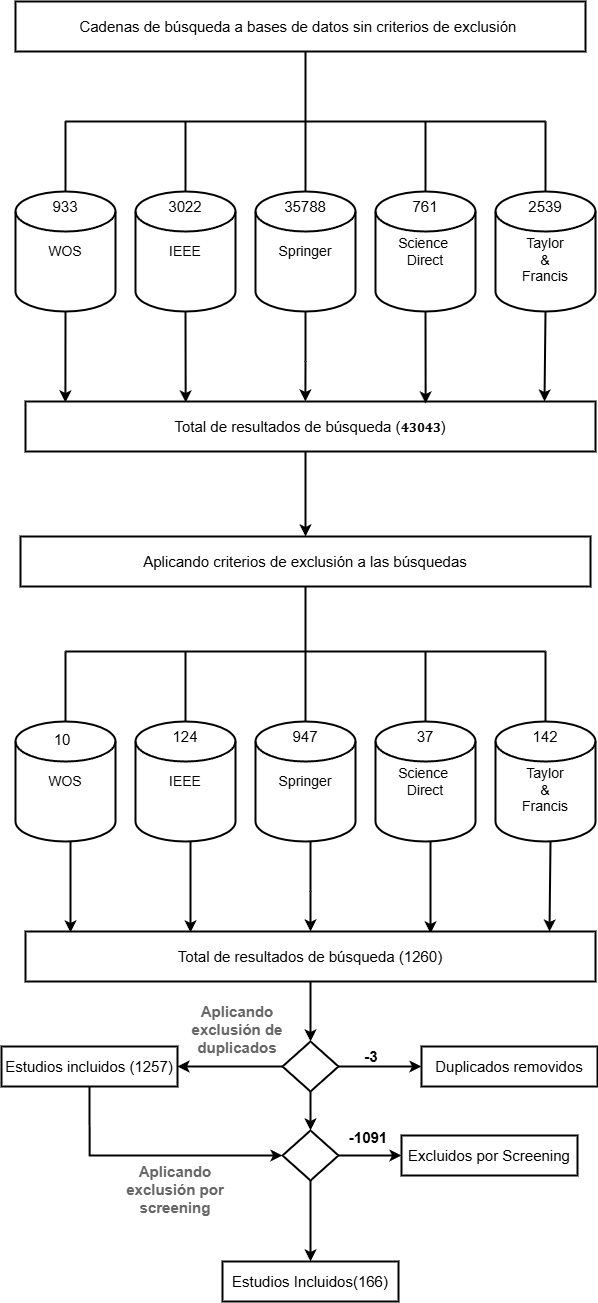
\includegraphics[scale=0.35]{resources/images/Planeacion/overview.png}
	\caption{Vista general de las actividades y resultados obtenidos en la estrategia de búsqueda por bases de datos}\label{fig:overview}
\end{figure}


\begin{table*}[htbp]
	\centering
	\begin{tabular}{p{4.8cm}p{1.7cm}p{1.7cm}p{1.7cm}p{1.7cm}p{2cm}p{1.4cm}}
		\toprule
		\textbf{Criterios}                                        & \textbf{ACM} & \textbf{IEEE} & \textbf{ScienceDirect} & \textbf{Springer} & \textbf{Taylor \& Francis} & \textbf{Total} \\
		\midrule
		\textbf{Cadena de búsqueda con palabras clave únicamente} & \iwos{}      & \iieee{}      & \isd{}                 & \ispr{}           & \itf{}                     & \itot{}        \\
		\addlinespace[0.8em]
		\textbf{Contribución porcentual}                          & \iwosp{}\%   & \iieeep{}\%   & \isdp{}\%              & \isprp{}\%        & \itfp{}\%                  & 100\%          \\
		\bottomrule
		\vspace{2pt}
	\end{tabular}
	\caption{Resultados de las cadenas de búsqueda con criterios de exclusión}\label{table:search_results_exclusion}
\end{table*}
% --------------------------------------------------------------


% sub-subsetion for 4.2.2 --- BUSQUEDA POR SNOWBALL 
% sub-subsetion for 4.2.2 ----- ESTRATEGIA DE BUSQUEDA POR SNOWBALL
\subsubsection{Estrategia de Búsqueda 2: Bola de nieve}

\newcommand{\firstBackwardSnowballStudies}{8} %Primera iteración hacia atrás
\newcommand{\firstForwardSnowballStudies}{7} % Primera iteración hacia adelante

%Total de estudios
\newcommand{\snowballNewStudies}{\fpeval{\firstBackwardSnowballStudies+\firstForwardSnowballStudies}}

La estrategia de búsqueda mediante \textit{snowballing} se aplicó con el objetivo de identificar estudios adicionales que pudieran 
no haber sido recuperados durante la búsqueda automática en las bases de datos. Siguiendo las recomendaciones metodológicas de 
Wohlin~\cite{Wohlin-01}, se consideraron tanto la bola de nieve inversa, basada en el análisis de las listas de referencias de los 
estudios seleccionados, como la bola de nieve directa, que consiste en identificar los trabajos que citan dichos estudios. Para este 
propósito se utilizó Google Académico como motor de búsqueda para el rastreo de citas.

% Snowball baseline building 
\bolditalic{Construcción de la base de la bola de nieve}: 
Como diferenciador metodológico, en este trabajo la estrategia de \textit{snowballing} se aplicó sobre la totalidad de los 166 
estudios seleccionados tras el proceso de selección, en lugar de emplear un conjunto reducido de artículos base (semilla). Esta 
decisión permitió ampliar la cobertura de la revisión y disminuir el riesgo de omitir literatura relevante, fortaleciendo la 
exhaustividad del protocolo.

\bolditalic{Selección de estudios}: 
A partir de los 166 estudios semilla se aplicaron las estrategias de bola de nieve directa e inversa con el objetivo de identificar 
literatura adicional relevante que no hubiera sido recuperada durante la búsqueda automática en las bases de datos. Los estudios 
identificados mediante este proceso fueron evaluados aplicando los mismos criterios de inclusión y exclusión definidos en la 
Tabla~\ref{table:inclusion_exclusion_criteria}, garantizando así la consistencia y rigurosidad del proceso de selección dentro del 
estudio de mapeo sistemático.

\begin{figure}[htbp]
	\centering
	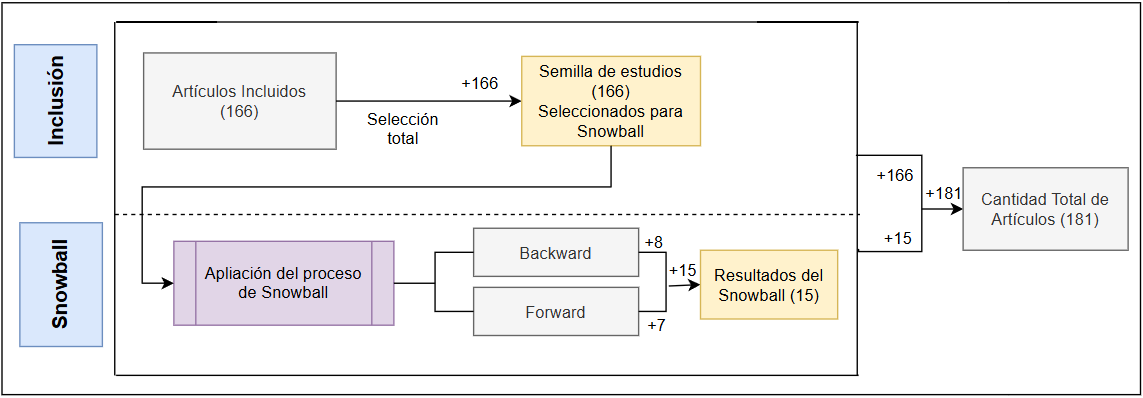
\includegraphics[scale=0.30]{resources/images/Planeacion/proceso_snowball.png}
	\caption{Estrategica de Busqueda Snowball.}\label{figure:Snowball}
\end{figure}

Esta actividad se realizó a través de Google Scholar, siguiendo la práctica del estudio~\cite{Ali-01}. El resultado obtenido fue 
\snowballNewStudies{} nuevos estudios. Cabe destacar que lo presentado en esta sección y en la Figura\ref{figure:Snowball} es un resumen 
representativo del proceso de bola de nieve; sin embargo, se omiten los pasos realizados que no contribuyen al objetivo del estudio. 
Por ejemplo, durante el proceso de bola de nieve se identificaron estudios que no cumplían con los criterios de inclusión, como libros y 
duplicados. Estos estudios fueron descartados y no se incluyeron en el conteo final de nuevos estudios obtenidos a través del proceso de 
bola de nieve.

% -------- Table : Inclusion/exclusion criteria ------------
\begin{table}[htbp]
	\centering
	\renewcommand{\arraystretch}{1}  % Increase row height globally
	\begin{tabular}{p{1.5cm}p{2.2cm}p{3.9cm}}
		\toprule
		\textbf{Category}         & \textbf{Inclusion} & \textbf{Exclusion}                                                                                           \\
		\midrule
		\textbf{Publication type} & Journal articles, Chapters  & Technical report, Conference proceedings and Thesis. \\
		\addlinespace[0.8em]
		\textbf{Period}           & From 2020 to 2026  & Less than 2020                                                                                                \\
		\addlinespace[0.8em]
		\textbf{Language}         & English            & ---                                                                                                              \\
		\bottomrule
		\vspace{1pt}
	\end{tabular}
	\caption{Criterios de Inclusion/exclusion Snowball}\label{table:inclusion_exclusion_criteria}
\end{table}
% --------------------------------------------------------------


% sub-subsetion for 4.2.3 -- RESULTADOS DE LA BUSQUEDA DE ESTUDIOS
%sub-subseccion 4.2.3 
\subsubsection{Resultados de la Búsqueda de Estudios}\label{subsubsec:resultados-busqueda}

\newcommand{\totalEtapaDos}{\fpeval{\screenTot+\snowballNewStudies}}
\newcommand{\dbPercentEtapa}{\fpeval{round (\screenTot*100/\totalEtapaDos,2)}}
\newcommand{\snowPercentEtapa}{\fpeval{round (\snowballNewStudies*100/\totalEtapaDos,2)}}

Finalmente, al sumar los estudios \snowballNewStudies{} obtenidos en el proceso de bola de nieve al \screenTot{} 
obtenido previamente con la estrategia de búsqueda en la base de datos, se obtiene un total de \totalEtapaDos{} 
estudios para esta etapa. Véase la Tabla~\ref{table:resultados_etapa_2}.

% -------- Table : Results of stage 2: Study search ------------
\begin{table}[htbp]
	\centering
	\renewcommand{\arraystretch}{1}  % Increase row height globally
	\begin{tabular}{p{2.5cm}p{2.6cm}p{2.5cm}}
		\toprule
		\textbf{Strategy} & \textbf{Studies}      & \textbf{\%}           \\
		\midrule
		Databases         & \screenTot{}          & \dbPercentEtapa{}\%   \\
		\addlinespace[0.8em]
		Snowballing       & \snowballNewStudies{} & \snowPercentEtapa{}\% \\
		\addlinespace[0.8em]
		Total             & \totalEtapaDos{}      &  100\%                 \\
		\bottomrule
		\vspace{2pt}
	\end{tabular}
	\caption{Results of stage 2: Search for studies}\label{table:resultados_etapa_2}
\end{table}
% --------------------------------------------------------------

%subsección 4.3
% subsection 4.3
\subsubsection{Etapa 3: Evaluación de calidad}

De acuerdo con la literatura sobre estudios de mapeo sistemático como el de~\cite{Ali-01} y~\cite{Petersen2008}, la evaluación de calidad 
no es un requisito obligatorio en este tipo de investigaciones; sin embargo, su incorporación permite aumentar la rigurosidad del proceso 
de selección y análisis de estudios. Por esta razón, en este trabajo se realizó una evaluación de calidad con el objetivo de verificar la 
relevancia y el impacto de los estudios identificados en relación con los objetivos del SMS.\@

Para llevar a cabo esta evaluación se utilizaron los índices CVI (\textit{Content Validity Index}), SCI (\textit{Study Citation Index})
e IRRQ (\textit{Index of Relationship to Research Questions}), los cuales fueron definidos y descritos en detalle durante la fase
de planificación (Sección~\ref{subsec:criterios_calidad}). Los valores de estos índices fueron calculados con el apoyo de la herramienta
SMS-Builder~\cite{Candela-Uribe2022}.

%sub-subsection 4.3.1
\subsubsection{Evaluación de validez del contenido}

En esta etapa se analizó el contenido de los estudios seleccionados con el fin de determinar su valor dentro del contexto de la 
investigación. Para ello se aplicó el índice CVI, el cual permite evaluar la relevancia del contenido de cada estudio respecto al 
dominio de investigación analizado.

Posteriormente, se efectuó un análisis de frecuencia para identificar el cuartil de estudios más significativos, es decir, aquellos 
con los valores más altos del índice CVI.\@ La definición formal de esta métrica se presenta en la 
Sección~\ref{subsec:criterios_calidad}, específicamente en la Ecuación~\ref{eq:cvi}.

%sub-subsection 4.3.2
\subsubsection{Índice de calidad basado en el número de citas}

La evaluación del impacto científico de los estudios se realizó mediante el índice SCI.\@ Este índice considera el número de citas
recibidas por cada publicación como un indicador de su influencia dentro de la comunidad académica.

El cálculo del índice SCI se realizó utilizando SMS-Builder en conjunto con los datos de citación obtenidos a partir de
Google Académico. Posteriormente,se llevó a cabo un análisis de frecuencia orientado a identificar el cuartil de estudios con 
mayor relevancia según este indicador. La formulación formal de esta métrica se presenta en la Sección~\ref{subsec:criterios_calidad}, 
específicamente en la Ecuación~\ref{eq:sci}.

%sub-subsection 4.3.3
\subsubsection{Relación de los estudios con las preguntas de investigación}

Finalmente, se aplicó el índice IRRQ con el fin de evaluar el grado de relación entre los estudios seleccionados y las preguntas de
investigación planteadas en este estudio.

Para ello, la herramienta SMS-Builder fue configurada para establecer la relación directa entre cada estudio y los temas de clasificación
definidos en el SMS.\@ Como en los casos anteriores, se realizó un análisis de frecuencia que permitió identificar el cuartil de
estudios con mayor relación con las preguntas de investigación. La formulación formal de esta métrica se presenta en la Sección~\ref{subsec:criterios_calidad}, 
específicamente en la Ecuación~\ref{eq:irrq}.

%subsección 4.4
% subseccion 4.4 ------- EXTRACCION DE DATOS
\subsection{Etapa 4: Extracción de datos}\label{sec:extraccion-de-datos}

Como resultado de la aplicación de los procedimientos de búsqueda, selección de estudios y evaluación de calidad, se identificó un 
total de \totalEtapaDos{} estudios primarios. Estos estudios se etiquetaron con el prefijo SPS (Estudio Primario Seleccionado) 
seguido de un número. La lista completa de estos estudios se puede encontrar en la Tabla~\ref{table:selected_primary_studies}. A 
partir de los \totalEtapaDos{} estudios primarios seleccionados, se diseño una taxonomía para completar uno de los objetivos 
planteados al inicio del SMS.\@ La información contenida en los SPS se relacionó con las preguntas de investigación a través de 
los temas definidos en la etapa de planificación y se registró utilizando los modelos GQM y PICOC.\@ Además, se extrajeron 
metadatos, como palabras clave, para identificar los aspectos subyacentes de los SPS.\@

% -------- Tabla : Estudios Primarios Seleccionados (SPSs) ------------
\begin{table*}[htbp]
	\centering
	\renewcommand{\arraystretch}{1.2}
	\setlength{\tabcolsep}{4pt} % Reduce space between columns
	\begin{tabular*}{\textwidth}{l @{\extracolsep{\fill}} r l @{\extracolsep{\fill}} r l @{\extracolsep{\fill}} r l @{\extracolsep{\fill}} r l @{\extracolsep{\fill}} r}
		\toprule
		\textbf{ID} & \textbf{Ref} 							& \textbf{ID} & \textbf{Ref} 								& \textbf{ID} & \textbf{Ref} 								& \textbf{ID} & \textbf{Ref} 								 & \textbf{ID} & \textbf{Ref} 						 	 \\
		\midrule
		SPS001      &~\cite{Nespoli2021}          			& SPS002      &~\cite{Robertson2022}         				& SPS003      &~\cite{Sharma2025}          					& SPS004      &~\cite{Aslam2024}          					 & SPS005      &~\cite{Pavithra2024}          		 	 \\
		SPS006      &~\cite{Jangjou2022}          			& SPS007      &~\cite{Gioiosa2025}          				& SPS008      &~\cite{Mohan2023}          					& SPS009      &~\cite{Vardhan2024}          				 & SPS010      &~\cite{Thakkar2023}         			 \\
		SPS011      &~\cite{Badie2023}   					& SPS012      &~\cite{Singh2025}       						& SPS013      &~\cite{Jimenez2021}         					& SPS014      &~\cite{Henriques2024}         				 & SPS015      &~\cite{Gupta2023}         			 	 \\
		SPS016      &~\cite{Bose2023HealthDataPrivacySurvey}& SPS017      &~\cite{Yu2020}  								& SPS018      &~\cite{Silva2025}         					& SPS019      &~\cite{Stoyanova2020} 						 & SPS020      &~\cite{Alsuwaiyan2025}         		 	 \\
		SPS021      &~\cite{Gill2024}         				& SPS022      &~\cite{Kumar2023IDS}         				& SPS023      &~\cite{Guerron2020}         					& SPS024      &~\cite{Zhukabayeva2024}         				 & SPS025      &~\cite{Rajesh2024}   				 	 \\
		SPS026      &~\cite{Ghanmi2025}         			& SPS027      &~\cite{Liu2021}         						& SPS028      &~\cite{Yu2025}         						& SPS029      &~\cite{Dahiya2024}         					 & SPS030      &~\cite{Akremi2021}     				 	 \\
		SPS031      &~\cite{Hozouri2025IDSsurvey}       	& SPS032      &~\cite{Khraisat2021IoTIDSReview}  			& SPS033      &~\cite{Kumar2025BlockchainHealthcare}		& SPS034      &~\cite{Marwan2020BlockchainIoT}      		 & SPS035      &~\cite{Mawgoud2022SteganographyCloud} 	 \\
		SPS036      &~\cite{Hu2024MetaheuristicIDS}      	& SPS037      &~\cite{Tariq2024FogEdgeIDS}         			& SPS038      &~\cite{Tiwari2025BlockchainHealthcareIPFS}   & SPS039      &~\cite{Saini2024HybridMLCloudPrivacy}		 & SPS040      &~\cite{Altherwi2025CloudEhealthSecurity} \\
		SPS041      &~\cite{Chen2025CloudAttackMitigation}  & SPS042      &~\cite{Kaur2023FogSecurityAHP} 				& SPS043      &~\cite{Merdassi2023LTMAABE}         			& SPS044      &~\cite{Thushara2023HybridEncryptionMedical}   & SPOX45      &~\cite{Kocaman2022CVEanalysis}         	 \\
		SPS046      &~\cite{Hasan2022BlockchainIIoT}        & SPS047      &~\cite{Reddy2025DLcloudSecurity}     		& SPS048      &~\cite{Wang2022ExtremeLearningIDS}         	& SPS049      &~\cite{Anilkumar2021AccessControlCloud}       & SPS050      &~\cite{Alam2022IoTauthentication}        \\
		SPS051      &~\cite{Adel2025ICTfailures}         	& SPS052      &~\cite{Kioskli2025HealthcareRiskFramework}   & SPS053      &~\cite{Lu2022CryptoBigDataSurvey}   			& SPS054      &~\cite{Raval2024CriticalInfrastructureSurvey} & SPS055      &~\cite{Tabrizchi2020CloudSecuritySurvey} \\
		SPS056      &~\cite{Nasim2025CloudIDSreview}        & SPS057      &~\cite{Kundiya2025InsiderThreatNLP}         	& SPS058      &~\cite{Edo2024ZeroTrustHealth}      			& SPS059      &~\cite{Almotiri2025AIoMTsecurity}      		 & SPS060      &~\cite{Alotaibi2025SDNIoTIDS}         	 \\
		SPS061      &~\cite{Sharma2025}         			& SPS062      &~\cite{Ouhssini2024DDoSCloudReview}      	& SPS063      &~\cite{Mallidi2025AIIDSIoT}      			& SPS064      &~\cite{Hussain2025WSNIDS}         			 & SPS065      &~\cite{Ray2023DDoSMHealth}         		 \\
		SPS066      &~\cite{Wedamuni2026CyberThreatIntel}   & SPS067      &~\cite{Lyu2025DPRKThreatLandscape}      		& SPS068      &~\cite{Songa2024SDNDDoS}         			& SPS069      &~\cite{Kure2022CyberRiskFramework}      		 & SPS070      &~\cite{Henge2023InsiderAttackDetection}  \\
		SPS071      &~\cite{Tian2025MalwarePropagationGame} & SPS072      &~\cite{Kaur2023AICybersecurityReview}        & SPS073      &~\cite{Choksy2023ABACIoTHealthcare}         	& SPS074      &~\cite{Yang2025BERTIDS}      				 & SPS075      &~\cite{Sable2025CloudThreatIntel}        \\
		SPS076      &~\cite{Islam2024ExplainableIDS}        & SPS077      &~\cite{Meriah2025SecurityOntology}         	& SPS078      &~\cite{Psathas2022COREM2}     				& SPS079      &~\cite{Sardar2025WoTSecurityReview}         	 & SPS080      &~\cite{Verma2020CloudStakeholder}        \\
		SPS081      &~\cite{Butt2023CloudSecuritySurvey}    & SPS082      &~\cite{Shahzad2022CloudAnomalyEnsemble}      & SPS083      &~\cite{Hadi2024CybersecurityToolsSurvey}     & SPS084      &~\cite{Tissir2021CloudCybersecurityManagement}& SPS085      &~\cite{Kanber2022ApplicationLayerDDoS}   \\
		SPS086      &~\cite{Aldweesh2020DeepLearningIDS}    & SPS087      &~\cite{Radoglou2022IIoTSecurity}      		& SPS088      &~\cite{Wang2022ExtremeLearningIDS}         	& SPS089      &~\cite{Kirubavathi2025TransformerDDoS}      	 & SPS090      &~\cite{Doğan2025SDNIDSReview}         	 \\
		SPS091      &~\cite{Obidallah2025RansomwareSMPC}    & SPS092      &~\cite{Kim2024CloudIDS}      				& SPS093      &~\cite{Belgacem2022CloudResourceTaxonomy}    & SPS094      &~\cite{Benmohamed2024ESDNN}         			 & SPS095      &~\cite{Kumar2025EdgeGuardIA}         	 \\
		SPS096      &~\cite{Chen2023SRUTabNetIDS}         	& SPS097      &~\cite{Rehman2025BlockchainIoTAuth}         	& SPS098      &~\cite{Folino2024FederatedLearning}      	& SPS099      &~\cite{Alansary2025AIThreats}         		 & SPS100      &~\cite{Ali2024CloudTrends}        		 \\
		SPS101      &~\cite{Reddy2024CloudEncryption}       & SPS102      &~\cite{Jalali2025Federated5GIoT}        		& SPS103      &~\cite{Swathi2025CloudAuthentication}      	& SPS104      &~\cite{Khan2024PrivacyAHP}      				 & SPS105      &~\cite{Zhang2025RansomwareDetection}     \\
		SPS106      &~\cite{Pinto2024InfrastructureSecurity}& SPS107      &~\cite{Saidi2025FederatedPrivacyIDS}        	& SPS108      &~\cite{Chatterjee2023CloudLMS}        		& SPS109      &~\cite{AlShehari2024InsiderThreat}        	 & SPS110      &~\cite{Sherin2026HybridIDS}        		 \\
		SPS111      &~\cite{Kandoussi2024BayesianDefense}   & SPS112      &~\cite{Preethi2025MultiCloudSecurity}        & SPS113      &~\cite{Quan2025SituationalAwareness}         & SPS114      &~\cite{Mani2025MemoryIDS}        			 & SPS115      &~\cite{Saeed2025CloudResilienceReview}   \\
		SPS116	    &~\cite{Mahboubi2024ThreatHuntingReview}& SPS117      &~\cite{Bhurani2025ExBCIL}     				& SPS118      &~\cite{Sarker2024ExplainableCybersecurity}   & SPS119      &~\cite{Gharbi2025IoTRansomwareSurvey}         & SPS120      &~\cite{RajeshKanna2024AttackDetection}   \\
		SPS121      &~\cite{Buyuktanir2025FederatedIDS}		& SPS122      &~\cite{Srinivasan2025FederatedCryptography}  & SPS123      &~\cite{Galle2025CyberResilienceBoard}        & SPS124      &~\cite{Du2025CostSensitiveTraffic}      		 & SPS125      &~\cite{Alotaibi2025SDNIoTIDS}        	 \\
		SPS126      &~\cite{Rana2024HeatmapAttacks}		 	& SPS127      &~\cite{Bouganim2023PrivacyQueries}         	& SPS128      &~\cite{Mamidala2025HybridCloudSecurity}      & SPS129      &~\cite{Vaneeta2026IDPSWOAXGBoost}         	 & SPS130      &~\cite{De2022ThreatModelingCloud}        \\
		SPS131      &~\cite{Pramudya2022SnortIDS}		 	& SPS132      &~\cite{Ecabert2024CyberIncidentReporting}	& SPS133      &~\cite{Alashjaee2024DigitalForensics}   		& SPS134      &~\cite{UlloaZamora2025MedicalDevicesSecurity} & SPS135      &~\cite{Mughaid2024IoTCloudSecurity}      \\
		SPS136      &~\cite{Dwivedi2024BibliometricIJIS}	& SPS137      &~\cite{Adiwal2023OpenStackIDS}         		& SPS138      &~\cite{Liu2022CloudIDSReview}      			& SPS139	  &~\cite{Pirbhulal2024IoT5GSecuritySLR}      	 & SPS140      &~\cite{Shukla2024IoTDDoSReview}          \\
		SPS141      &~\cite{Ammi2022CloudThreatIntelligence}& SPS142      &~\cite{Sophie2025MultiLayerSecurity}      	& SPS143      &~\cite{Mohammadi2025DenialWallet}      		& SPS144      &~\cite{Jaiswal2025InsiderThreatReview}		 & SPS145      &~\cite{Aboukadri2024IAMSurvey}        	 \\
		SPS146      &~\cite{Tebbaa2026SDNDDoSSLR}      		& SPS147      &~\cite{MartinezBeltran2024FederatedDefense}  & SPS148      &~\cite{Ullah2025ContentPoisoningSurvey}   	& SPS149      &~\cite{Bistene2025TrafficGeneratorsSLR}       & SPS150      &~\cite{Zhang2025CloudDatabaseSecurity}   \\
		SPS151      &~\cite{Bennaceur2026MultiDimTrust}		& SPS152      &~\cite{Henge2025MultiLayerAccessControl} 	& SPS153      &~\cite{Samah2024CyberespionageWFH}         	& SPS154      &~\cite{Gambo2025SaudiCybersecurity}      	 & SPS155      &~\cite{Zhao2024SituationalAwareness}     \\
		SPS156      &~\cite{Li2025ThreatDetectionFusion}	& SPS157      &~\cite{Benkhelifa2025NextGenPentesting}		& SPS158      &~\cite{Batra2025MultiCloudDataLoss}		 	& SPS159      &~\cite{Ting2021TrustModeling}         		 & SPS160      &~\cite{Kumar2025HPCCloudSLR}        	 \\
		SPS161      &~\cite{John2024DigitalTwinTrust}		& SPS162      &~\cite{Velmurugan2024SelectiveSharing}		& SPS163      &~\cite{Chen2021QShield}   					& SPS164      &~\cite{Ahmad2022CASBSLR}		 				 & SPS165      &~\cite{Ahamed2022OsqueryDetection}       \\
		SPS166      &~\cite{Alzoubi2024MLCloudSecurity}		& SPS167      &~\cite{Alqahtani2023CloudThreatReview}       & SPS168      &~\cite{Coppolino2022SIEMEHealth}      		& SPS169      &~\cite{Ardebili2024CyberResilience}      	 & SPS170      &~\cite{Chimuco2023MobileCloudSecurity}   \\
		SPS171      &~\cite{Kamble2025SecureIoTTransmission}& SPS172      &~\cite{Vijay2025TrustReputationCloud}      	& SPS173      &~\cite{ElKafhali2022CloudSecurityReview}     & SPS174      &~\cite{Vashishth2024CloudEducationSecurity}	 & SPS175      &~\cite{Nagarchi2025MultiCloudSecurity}   \\
		SPS176      &~\cite{Bader2023CyberThreatStudy}      & SPS177      &~\cite{Ray2021CloudIoTSecurity}		 		& SPS178      &~\cite{Wu2023SpaceNetworkThreats}   			& SPS179      &~\cite{Ullah2026CyberDefenseReview}      	 & SPS180      &~\cite{Stojalowski2024ZeroTrust}         \\
		SPS181      &~\cite{Ahmad2023ZeroDaySLR} 		 	& ---      	  & ---      									& ---      	  & ---         								& ---      	  & ---      									 & ---         & ---        							 \\
		\bottomrule
		\vspace{2pt}
	\end{tabular*}
	\caption{Los \totalStudies{} estudios primarios seleccionados (SPSs)}\label{table:selected_primary_studies}
\end{table*}
% --------------------------------------------------------------

El proceso se apoyó en diversas herramientas informáticas, como hojas de cálculo, software especializado para la gestión de referencias 
bibliográficas como Mendeley~\cite{mendeley} y SMS-Builder~\cite{Candela-Uribe2022} para la construcción del análisis de datos. Toda la información de 
este SMS se ha publicado en el sitio~\cite{sms_cloud_security_tg} y los métodos de acceso se describen en la sección~\ref{sec:reproducibilidad}.

%subsección 4.5

% subseccion 4.5
\subsection{Etapa 5: Clasificación de estudios}\label{subsec:clasificacion-de-estudios}
La clasificación del SPS se realizó mediante la agrupación por temas, como se muestra en la Tabla~\ref{table:sps_classification_by_topic_rq}. Esta tabla presenta un resumen de los estudios que responden a las preguntas de investigación RQ1 y RQ2.

% Tabla 13 V2 ----------CLASIFICACION SPSs POR PREGUNTA DE RQs y Tópicos
\begin{table*}[htbp]
	\centering
	\tiny
	\renewcommand{\arraystretch}{0.5}
	%\setlength{\tabcolsep}{0.9pt}
	\begin{tabularx}{\textwidth}{p{0.5cm}p{1.5cm}>{\raggedright\arraybackslash}X>{\raggedright\arraybackslash}X>{\raggedright\arraybackslash}X}
		\toprule
		\textbf{RQ}                           & \textbf{Topic}   	& \textbf{2023-2024}                         & \textbf{2025-2026}  						\\
		\midrule
		\multirow{0}{*}[-10em]{\textbf{RQ1}} & CLOUD 
												COMPUTING 		& SPS008 SPS010 SPS011 SPS015 SPS016 SPS022
																	  SPS042 SPS043 SPS044 SPS061 SPS065 SPS070 
																	  SPS072 SPS073 SPS081 SPS108 SPS127 SPS137 
																	  SPS167 SPS178 SPS181 SPS005 SPS009 SPS014 
																	  SPS021 SPS024 SPS025 SPS029 SPS036 SPS037 
																	  SPS039 SPS054 SPS058 SPS062 SPS068 SPS076 
																	  SPS083 SPS092 SPS094 SPS098 SPS100 SPS101 
																	  SPS104 SPS106 SPS111 SPS116 SPS120 SPS126 
																	  SPS132 SPS133 SPS135 SPS136 SPS147 SPS155 
																	  SPS161 SPS162 SPS180	     				 & SPS003 SPS007 SPS012 SPS018 SPS020 SPS026
																												   SPS028 SPS031 SPS033 SPS038 SPS040 SPS041 
																												   SPS047 SPS051 SPS052 SPS056 SPS057 SPS059 
																												   SPS060 SPS063 SPS064 SPS071 SPS074 SPS075 
																												   SPS087 SPS089 SPS090 SPS091 SPS099 SPS102 
																												   SPS103 SPS105 SPS107 SPS112 SPS113 SPS114 
																												   SPS115 SPS117 SPS119 SPS121 SPS122 SPS124 
																												   SPS125 SPS134 SPS142 SPS143 SPS149 SPS150 
																												   SPS151 SPS152 SPS154 SPS156 SPS157 SPS158 
																												   SPS160 SPS171 SPS172 SPS174 SPS175 SPS066 
																												   SPS129 SPS146 SPS179                        \\
		\addlinespace[0.3em]
		\cmidrule(lr){2-4}				  
		                                      & CYBER
											  	SECURITY         	& SPS008 SPS010 SPS011 SPS015 SPS016 SPS022 
																		  SPS042 SPS043 SPS044 SPS061 SPS065 SPS070 
																		  SPS072 SPS073 SPS081 SPS096 SPS108 SPS127 
																		  SPS137 SPS167 SPS170 SPS176 SPS178 SPS181	
																		  SPS004 SPS005 SPS009 SPS014 SPS021 SPS024 
																		  SPS025 SPS029 SPS036 SPS037 SPS039 SPS054 
																		  SPS058 SPS062 SPS068 SPS076 SPS083 SPS092 
																		  SPS094 SPS098 SPS100 SPS101 SPS104 SPS106 
																		  SPS109 SPS111 SPS116 SPS118 SPS120 SPS126 
																		  SPS132 SPS133 SPS135 SPS136 SPS139 SPS140 
																		  SPS145 SPS147 SPS153 SPS155 SPS161 SPS162 
																		  SPS166 SPS169 SPS180                       & SPS003 SPS007 SPS012 SPS018 SPS020 SPS026 
																													   SPS028 SPS031 SPS033 SPS038 SPS040 SPS041 
																													   SPS047 SPS051 SPS052 SPS056 SPS057 SPS059 
																													   SPS060 SPS063 SPS064 SPS067 SPS071 SPS074 
																													   SPS075 SPS079 SPS087 SPS089 SPS090 SPS091 
																													   SPS095 SPS097 SPS099 SPS102 SPS103 SPS105 
																													   SPS107 SPS112 SPS113 SPS114 SPS115 SPS117 
																													   SPS119 SPS121 SPS122 SPS123 SPS124 SPS125 
																													   SPS128 SPS134 SPS142 SPS143 SPS144 SPS148 
																													   SPS149 SPS150 SPS151 SPS152 SPS154 SPS156 
																													   SPS157 SPS158 SPS160 SPS171 SPS172 SPS174 
																													   SPS175 SPS066 SPS110 SPS129 SPS146 SPS179 \\
		\addlinespace[0.3em]
		\cmidrule(lr){2-4}
		                                      & SECURITY
											  	 CONTROLS       & SPS008 SPS010 SPS011 SPS015 SPS016 SPS022 
																		  SPS042 SPS043 SPS044 SPS061 SPS065 SPS070 
																		  SPS072 SPS073 SPS081 SPS096 SPS108 SPS127 
																		  SPS137 SPS167 SPS170 SPS178 SPS181 SPS004 
																		  SPS005 SPS009 SPS014 SPS021 SPS024 SPS025 
																		  SPS029 SPS036 SPS037 SPS039 SPS054 SPS058 
																		  SPS062 SPS068 SPS076 SPS083 SPS092 SPS094 
																		  SPS098 SPS100 SPS101 SPS104 SPS106 SPS111 
																		  SPS116 SPS118 SPS120 SPS126 SPS132 SPS133 
																		  SPS135 SPS136 SPS147 SPS153 SPS155 SPS161 
																		  SPS162 SPS180                               & SPS003 SPS007 SPS012 SPS018 SPS020 SPS026 
																														SPS028 SPS031 SPS033 SPS038 SPS040 SPS041 
																														SPS047 SPS051 SPS052 SPS056 SPS057 SPS059 
																														SPS060 SPS063 SPS064 SPS067 SPS071 SPS074 
																														SPS075 SPS077 SPS079 SPS087 SPS089 SPS090 
																														SPS091 SPS095 SPS097 SPS099 SPS102 SPS103 
																														SPS105 SPS107 SPS112 SPS113 SPS114 SPS115 
																														SPS117 SPS119 SPS121 SPS122 SPS124 SPS125 
																														SPS134 SPS142 SPS143 SPS148 SPS149 SPS150 
																														SPS151 SPS152 SPS154 SPS156 SPS157 SPS158 
																														SPS160 SPS172 SPS174 SPS175 SPS066 SPS110 
																														SPS129 SPS146 SPS179                      \\
		\addlinespace[0.3em]
		\cmidrule(lr){2-4}
		                                      & ARCHITECTURE          	& SPS016 SPS042 SPS044 SPS061 SPS065 SPS070 
																		  SPS081 SPS108 SPS127 SPS137 SPS170 SPS176 
																		  SPS178 SPS004 SPS014 SPS024 SPS029 SPS054 
																		  SPS058 SPS062 SPS076 SPS098 SPS101 SPS104 
																		  SPS111 SPS116 SPS118 SPS133 SPS135 SPS139 
																		  SPS140 SPS145 SPS147 SPS155 SPS161 SPS162 
																		  SPS180 										& SPS003 SPS007 SPS012 SPS018 SPS020 SPS026 
																														  SPS031 SPS041 SPS051 SPS056 SPS057 SPS059 
																														  SPS060 SPS063 SPS071 SPS074 SPS075 SPS079 
																														  SPS089 SPS090 SPS091 SPS102 SPS103 SPS107 
																														  SPS112 SPS119 SPS121 SPS124 SPS142 SPS144 
																														  SPS149 SPS150 SPS151 SPS156 SPS157 SPS158 
																														  SPS160 SPS171 SPS174 SPS175 SPS066 SPS129 
																														  SPS146 SPS179                      		\\
		\addlinespace[0.3em]
		\cmidrule(lr){2-4}
		                                      & ISO/IEC 27001           & SPS008 SPS010 SPS011 SPS015 SPS016 SPS022 
																		  SPS042 SPS043 SPS044 SPS061 SPS065 SPS070 
																		  SPS072 SPS073 SPS081 SPS096 SPS108 SPS127 
																		  SPS137 SPS167 SPS170 SPS178 SPS004 SPS005 
																		  SPS009 SPS014 SPS021 SPS024 SPS025 SPS029 
																		  SPS036 SPS037 SPS039 SPS054 SPS058 SPS062 
																		  SPS068 SPS076 SPS092 SPS094 SPS098 SPS101 
																		  SPS104 SPS111 SPS118 SPS120 SPS126 SPS132 
																		  SPS133 SPS135 SPS136 SPS139 SPS140 SPS145 
																		  SPS147 SPS153 SPS155 SPS161 SPS162 SPS169 
																		  SPS180  									& SPS003 SPS007 SPS012 SPS018 SPS020 SPS026 
																													  SPS028 SPS031 SPS033 SPS040 SPS041 SPS047 
																													  SPS051 SPS052 SPS056 SPS057 SPS059 SPS060 
																													  SPS063 SPS064 SPS067 SPS071 SPS074 SPS075 
																													  SPS077 SPS079 SPS087 SPS089 SPS090 SPS091 
																													  SPS095 SPS102 SPS103 SPS105 SPS107 SPS112 
																													  SPS113 SPS114 SPS117 SPS119 SPS122 SPS123 
																													  SPS124 SPS125 SPS134 SPS142 SPS144 SPS149 
																													  SPS150 SPS151 SPS152 SPS154 SPS158 SPS160 
																													  SPS171 SPS174 SPS175 SPS066 SPS110 SPS129 
																													  SPS146 									\\
		\addlinespace[0.3em]
		\cmidrule(lr){2-4}
		                                      & SECURITY                & SPS008 SPS010 SPS011 SPS015 SPS016 SPS022 
																		  SPS042 SPS043 SPS044 SPS065 SPS070 SPS072 
																		  SPS073 SPS081 SPS096 SPS108 SPS127 SPS137 
																		  SPS167 SPS170 SPS178 SPS181 SPS004 SPS005 
																		  SPS009 SPS014 SPS024 SPS025 SPS029 SPS036 
																		  SPS037 SPS039 SPS054 SPS058 SPS062 SPS068 
																		  SPS076 SPS083 SPS092 SPS094 SPS098 SPS100 
																		  SPS101 SPS106 SPS111 SPS120 SPS126 SPS133 
																		  SPS135 SPS147 SPS155 SPS161 SPS180     	& SPS003 SPS012 SPS018 SPS020 SPS026 SPS028 
																													  SPS031 SPS033 SPS038 SPS040 SPS041 SPS047 
																													  SPS051 SPS052 SPS056 SPS057 SPS059 SPS060 
																													  SPS063 SPS064 SPS067 SPS071 SPS074 SPS075 
																													  SPS077 SPS079 SPS087 SPS089 SPS090 SPS091 
																													  SPS095 SPS097 SPS099 SPS102 SPS103 SPS107 
																													  SPS112 SPS113 SPS114 SPS115 SPS117 SPS119 
																													  SPS121 SPS124 SPS125 SPS134 SPS142 SPS148 
																													  SPS150 SPS151 SPS152 SPS154 SPS156 SPS158 
																													  SPS160 SPS171 SPS172 SPS174 SPS175 SPS066 
																													  SPS110 SPS129 SPS146                       \\
		
		\addlinespace[0.3em]
		\cmidrule(lr){2-4}
											  & SECURITY INFORMATION 
											  AND EVENT MANAGEMENT (SIEM) & SPS008 SPS010 SPS011 SPS016 SPS022 SPS042 
																			SPS044 SPS072 SPS081 SPS108 SPS137 SPS167 
																			SPS178	SPS005 SPS009 SPS021 SPS024 SPS025 
																			SPS036 SPS039 SPS054 SPS058 SPS062 SPS068 
																			SPS076 SPS083 SPS098 SPS100 SPS101 SPS104 
																			SPS111 SPS126 SPS132 SPS133 SPS135 SPS155 
																			SPS161 SPS169 SPS180						& SPS007 SPS018 SPS026 SPS028 SPS033 SPS038 
																														  SPS040 SPS041 SPS047 SPS051 SPS052 SPS056 
																														  SPS057 SPS059 SPS060 SPS064 SPS067 SPS071 
																														  SPS074 SPS075 SPS087 SPS089 SPS090 SPS102 
																														  SPS103 SPS107 SPS112 SPS113 SPS115 SPS117 
																														  SPS119 SPS122 SPS124 SPS125 SPS134 SPS152 
																														  SPS154 SPS156 SPS157 SPS171 SPS172 SPS174 
																														  SPS175 SPS129 SPS179						 \\																														  \midrule %-----------------------------------------------------------------------------------------------------------------------------------------------------------------------------------------------------------------------
		\multirow{3}{*}[-2em]{\textbf{RQ2}}   & CLOUD COMPUTING         & SPS008 SPS010 SPS011 SPS015 SPS016 SPS022 
																		  SPS042 SPS043 SPS044 SPS061 SPS065 SPS070 
																		  SPS072 SPS073 SPS081 SPS108 SPS127 SPS137 
																		  SPS167 SPS170 SPS178 SPS181 SPS004 SPS005 
																		  SPS009 SPS014 SPS021 SPS024 SPS025 SPS029 
																		  SPS036 SPS037 SPS039 SPS054 SPS058 SPS062 
																		  SPS068 SPS076 SPS083 SPS092 SPS098 SPS100 
																		  SPS101 SPS104 SPS111 SPS116 SPS118 SPS120 
																		  SPS126 SPS133 SPS135 SPS136 SPS139 SPS140 
																		  SPS145 SPS147 SPS155 SPS161 SPS162 SPS169 
																		  SPS18           							 & SPS003 SPS007 SPS012 SPS018 SPS020 SPS026 
																													   SPS028 SPS031 SPS033 SPS038 SPS040 SPS041 
																													   SPS047 SPS051 SPS052 SPS056 SPS057 SPS059 
																													   SPS060 SPS063 SPS064 SPS067 SPS071 SPS074 
																													   SPS075 SPS079 SPS087 SPS089 SPS090 SPS091 
																													   SPS099 SPS102 SPS103 SPS107 SPS112 SPS113 
																													   SPS114 SPS115 SPS117 SPS119 SPS121 SPS122 
																													   SPS123 SPS124 SPS125 SPS134 SPS142 SPS144 
																													   SPS149 SPS150 SPS151 SPS154 SPS156 SPS157 
																													   SPS158 SPS160 SPS171 SPS172 SPS174 SPS175	
																													   SPS066 SPS110 SPS129 SPS146 SPS179 		  \\
		\addlinespace[0.3em]
		\cmidrule(lr){2-4}
		                                      & TAXONOMY                & SPS008 SPS010 SPS011 SPS015 SPS016 SPS022 
																		  SPS042 SPS043 SPS044 SPS061 SPS065 SPS070 
																		  SPS072 SPS073 SPS081 SPS096 SPS108 SPS127 
																		  SPS137 SPS167 SPS170 SPS176 SPS178 SPS181	
																		  SPS004 SPS005 SPS009 SPS014 SPS021 SPS024 
																		  SPS025 SPS029 SPS036 SPS037 SPS039 SPS054 
																		  SPS058 SPS062 SPS068 SPS076 SPS083 SPS092 
																		  SPS094 SPS098 SPS100 SPS101 SPS104 SPS106 
																		  SPS111 SPS116 SPS118 SPS120 SPS126 SPS132 
																		  SPS133 SPS135 SPS136 SPS139 SPS140 SPS145 
																		  SPS147 SPS155 SPS161 SPS162 SPS169 SPS180   & SPS003 SPS007 SPS012 SPS018 SPS020 SPS026 
																													   	SPS028 SPS031 SPS033 SPS038 SPS040 SPS041 
																														SPS047 SPS051 SPS052 SPS056 SPS057 SPS059 
																														SPS060 SPS063 SPS064 SPS067 SPS071 SPS074 
																														SPS075 SPS077 SPS079 SPS087 SPS089 SPS090 
																														SPS091 SPS095 SPS099 SPS102 SPS103 SPS105 
																														SPS107 SPS112 SPS113 SPS114 SPS115 SPS117 
																														SPS119 SPS121 SPS122 SPS123 SPS124 SPS125 
																														SPS134 SPS142 SPS143 SPS144 SPS149 SPS150 
																														SPS151 SPS152 SPS154 SPS156 SPS157 SPS160 
																														SPS171 SPS172 SPS174 SPS175 SPS066 SPS110 
																														SPS129 SPS146 SPS179  						\\
		\addlinespace[0.3em]
		\cmidrule(lr){2-4}
		                                      & ARCHITECTURE            & SPS008 SPS010 SPS011 SPS015 SPS016 SPS022 
																		 SPS042 SPS043 SPS044 SPS061 SPS065 SPS070 
																		 SPS072 SPS073 SPS081 SPS096 SPS108 SPS127 
																		 SPS137 SPS167 SPS176 SPS178 SPS181 SPS005 
																		 SPS009 SPS014 SPS021 SPS024 SPS025 SPS029 
																		 SPS036 SPS037 SPS039 SPS054 SPS058 SPS062 
																		 SPS068 SPS076 SPS083 SPS092 SPS094 SPS098 
																		 SPS100 SPS101 SPS104 SPS106 SPS109 SPS111 
																		 SPS116 SPS118 SPS120 SPS126 SPS132 SPS133 
																		 SPS135 SPS136 SPS139 SPS147 SPS153 SPS155 
																		 SPS161 SPS162 SPS166 SPS169 SPS180         & SPS003 SPS007 SPS012 SPS018 SPS020 SPS026 
																													  SPS028 SPS031 SPS033 SPS038 SPS040 SPS041 
																													  SPS047 SPS051 SPS052 SPS056 SPS057 SPS059 
																													  SPS060 SPS063 SPS064 SPS067 SPS071 SPS074 
																													  SPS075 SPS079 SPS087 SPS089 SPS090 SPS091 
																													  SPS095 SPS097 SPS099 SPS102 SPS103 SPS105 
																													  SPS107 SPS112 SPS113 SPS114 SPS115 SPS117 
																													  SPS119 SPS121 SPS122 SPS123 SPS124 SPS125 
																													  SPS128 SPS134 SPS142 SPS143 SPS144 SPS149 
																													  SPS150 SPS151 SPS152 SPS154 SPS156 SPS157 
																													  SPS158 SPS160 SPS171 SPS172 SPS174 SPS175	
																													  SPS066 SPS110 SPS129 SPS146 SPS179         \\
		\addlinespace[0.3em]
		\cmidrule(lr){2-4}
											  & SECURITY            	& SPS008 SPS010 SPS011 SPS015 SPS016 SPS022 
																		  SPS042 SPS043 SPS044 SPS061 SPS065 SPS070 
																		  SPS073 SPS081 SPS096 SPS108 SPS127 SPS137 
																		  SPS167 SPS170 SPS176 SPS178 SPS181 SPS004 
																		  SPS005 SPS009 SPS014 SPS024 SPS029 SPS036 
																		  SPS037 SPS039 SPS054 SPS058 SPS062 SPS076 
																		  SPS083 SPS092 SPS094 SPS098 SPS100 SPS101 
																		  SPS104 SPS106 SPS111 SPS116 SPS118 SPS120 
																		  SPS126 SPS132 SPS133 SPS135 SPS139 SPS140 
																		  SPS145 SPS147 SPS155 SPS161 SPS169 SPS180  & SPS003 SPS007 SPS012 SPS018 SPS020 SPS026 
																													   SPS031 SPS033 SPS038 SPS041 SPS047 SPS051 
																													   SPS052 SPS056 SPS057 SPS059 SPS060 SPS063 
																													   SPS064 SPS074 SPS075 SPS077 SPS079 SPS089 
																													   SPS090 SPS091 SPS095 SPS097 SPS099 SPS102 
																													   SPS103 SPS105 SPS107 SPS112 SPS113 SPS114 
																													   SPS115 SPS117 SPS119 SPS121 SPS124 SPS134 
																													   SPS142 SPS143 SPS144 SPS148 SPS149 SPS150 
																													   SPS151 SPS152 SPS154 SPS156 SPS158 SPS160 
																													   SPS172 SPS174 SPS175 SPS066 SPS110 SPS129 
																													   SPS146                                     \\
		\addlinespace[0.3em]
		\cmidrule(lr){2-4}
											  & CLASSIFICATION          & SPS008 SPS010 SPS011 SPS016 SPS022 SPS042 
																		  SPS044 SPS061 SPS065 SPS070 SPS072 SPS073 
																		  SPS081 SPS096 SPS108 SPS127 SPS170 SPS176 
																		  SPS178 SPS181 SPS004 SPS005 SPS009 SPS014 
																		  SPS021 SPS024 SPS025 SPS029 SPS037 SPS039 
																		  SPS054 SPS058 SPS062 SPS068 SPS076 SPS083 
																		  SPS092 SPS094 SPS098 SPS100 SPS101 SPS104 
																		  SPS106 SPS111 SPS116 SPS118 SPS126 SPS132 
																		  SPS133 SPS135 SPS136 SPS139 SPS140 SPS145 
																		  SPS147 SPS155 SPS161 SPS162 SPS169 SPS180   & SPS003 SPS007 SPS012 SPS018 SPS020 SPS026 
																														SPS028 SPS031 SPS033 SPS038 SPS040 SPS041 
																														SPS051 SPS052 SPS056 SPS057 SPS059 SPS060 
																														SPS063 SPS064 SPS071 SPS074 SPS075 SPS079 
																														SPS087 SPS089 SPS090 SPS091 SPS095 SPS099 
																														SPS102 SPS103 SPS105 SPS107 SPS112 SPS113 
																														SPS114 SPS115 SPS117 SPS119 SPS121 SPS124 
																														SPS125 SPS134 SPS142 SPS143 SPS144 SPS149 
																														SPS150 SPS151 SPS152 SPS154 SPS156 SPS157 
																														SPS158 SPS160 SPS171 SPS172 SPS174 SPS175	
																														SPS066 SPS110 SPS129 SPS146 SPS179         \\
		\addlinespace[0.3em]
		\cmidrule(lr){2-4}
											  & ZERO-TRUST				& SPS008 SPS010 SPS022 SPS042 SPS044 SPS065 
																		  SPS070 SPS081 SPS096 SPS127 SPS137 SPS167 
																		  SPS178 SPS014 SPS021 SPS024 SPS025 SPS029 
																		  SPS036 SPS039 SPS058 SPS062 SPS076 SPS094 
																		  SPS098 SPS101 SPS104 SPS111 SPS126 SPS132 
																		  SPS133 SPS135 SPS155 SPS161 SPS169 SPS180	 & SPS007 SPS012 SPS026 SPS028 SPS031 SPS033 
																													   SPS040 SPS041 SPS047 SPS052 SPS060 SPS063 
																													   SPS075 SPS089 SPS095 SPS103 SPS105 SPS107 
																													   SPS112 SPS122 SPS142 SPS150 SPS151 SPS152 
																													   SPS154 SPS160 SPS171 SPS174 SPS175 SPS066 
																													   SPS110 SPS129 SPS146						 \\
	\bottomrule
	\vspace{2pt}
	\end{tabularx}
	\caption{Classification of SPSs by topics and RQs}\label{table:sps_classification_by_topic_rq}
\end{table*}
% ------------------------------------------------------------------------

La agrupación de estudios por temas implica que un mismo SPS puede estar relacionado con uno o más. Por ejemplo, los estudios como el SPS097 y entre otros más se relacionan con ambas preguntas de investigación pero en temas especificos.
Tras esta clasificación inicial, los SPS se evaluaron según criterios de inclusión/exclusión y criterios de calidad, como los índices CVI, SCI e IRRQ.\@ Los criterios utilizados para el análisis y la clasificación de los SPS coinciden con los criterios de calidad. Véase las tablas~\ref{table:highest_CVI},~\ref{table:highest_SCI} y~\ref{table:highest_IRRQ}.
Tras comprender la composición del conjunto SPS y su calidad según los criterios mencionados, procedemos a proponer una relación entre los temas propuestos en la Tabla~\ref{table:sps_classification_by_topic_rq}, las meodologías y tecnlogías de seguridad en la nube hasta la fecha. Véase la Tabla~\ref{table:topics_metodology_tecnologies}.
Así, por ejemplo, un lector interesado en cualquier metodología o tecnología de seguridad en la nube podría consultar la Tabla~\ref{table:topics_metodology_tecnologies}, ver los temas más relacionados con este Universo y, a continuación, acceder a la Tabla~\ref{table:sps_classification_by_topic_rq} para consultar los estudios que se refieren a cada uno de estos temas y, transitivamente, al tema de interés. De igual modo, si el lector interesado en cualquier metodología o tecnología de seguridad desea consultar únicamente los estudios más relevantes relacionados con un tema determinado según su SCI, puede consultar la Tabla~\ref{table:highest_SCI}. De ahí el valor de esta correlación.
Cabe aclarar que es posible que alguna metodología o tecnología no tenga una relación directa con ningún dominio de seguridad o computación en la nube, por lo que se decide no mostrarlo. De igual manera, puede haber estudios que mantengan alguna relación con más de un tema; por lo tanto, se decide mostrar el tema con el que esté más estrechamente relacionado. De esta manera, la información que se muestra en la Tabla~\ref{table:topics_metodology_tecnologies} es más directa y concisa.

% Tabla 14 ---------------- tabla de estudios clasificados por CVI y Clasificación por tópicos

\begin{table*}[htbp]
	\centering
	%\renewcommand{\arraystretch}{2.0}
	\setlength{\tabcolsep}{2pt}
	\begin{tabularx}{\textwidth}{p{0.8cm}p{2.5cm}>{\raggedright\arraybackslash}X>{\raggedright\arraybackslash}X}
		\toprule
		\textbf{RQ}                          & \textbf{Topic}  & \textbf{2023-2024}                         	& \textbf{2025-2026}                                         \\
		\midrule
		\multirow{0}{*}[0em]{\textbf{RQ1}}  & CLOUD COMPUTING  & SPS008 SPS010 SPS011 SPS016 SPS022 SPS042 
																 SPS043 SPS070 SPS081 SPS137 SPS181 SPS014 
																 SPS021 SPS024 SPS025 SPS029 SPS036 SPS062 
																 SPS092 SPS100 SPS180                   		& SPS012 SPS018 SPS028 SPS033 SPS041 SPS047 
																												  SPS090 SPS142 SPS152 SPS174 SPS179                          \\
		\addlinespace[0.3em]
		\cmidrule(lr){2-4}	
		                                     & CYBERSECURITY 	& SPS008 SPS010 SPS011 SPS016 SPS022 SPS042 
																  SPS043 SPS070 SPS081 SPS137 SPS181 SPS014 
																  SPS021 SPS024 SPS025 SPS029 SPS036 SPS062 
																  SPS092 SPS100 SPS180                   		& SPS012 SPS018 SPS028 SPS033 SPS041 SPS047 
																												  SPS090 SPS142 SPS152 SPS174 SPS179             		      \\
		\addlinespace[0.3em]
		\cmidrule(lr){2-4}	
		                                     & SECURITY CONTROLS & SPS008 SPS010 SPS011 SPS016 SPS022 SPS042 
																   SPS043 SPS070 SPS081 SPS137 SPS181 SPS014 
																   SPS021 SPS024 SPS025 SPS029 SPS036 SPS062 
																   SPS092 SPS100 SPS180                       & SPS012 SPS018 SPS028 SPS033 SPS041 SPS047 
																												SPS077 SPS090 SPS142 SPS152 SPS174 SPS179            	   \\
		\addlinespace[0.3em]
		\cmidrule(lr){2-4}	
		                                     & ARCHITECTURE       & SPS016 SPS042 SPS070 SPS081 SPS137 SPS014 
																	SPS024 SPS029 SPS062 SPS180             	 & SPS012 SPS018 SPS041 SPS090 SPS142 SPS174 
																												   SPS179                        							\\
		\addlinespace[0.3em]
		\cmidrule(lr){2-4}	
		                                     & ISO/IEC 27001   	  & SPS008 SPS010 SPS011 SPS016 SPS022 SPS042 
																	SPS043 SPS070 SPS081 SPS137	SPS014 SPS021 
																	SPS024 SPS025 SPS029 SPS036 SPS062 SPS092 
																	SPS180             							  & SPS012 SPS018 SPS028 SPS033 SPS041 SPS047 
																													SPS077 SPS090 SPS142 SPS152 SPS174                            \\
		\addlinespace[0.3em]
		\cmidrule(lr){2-4}	
		                                     & SECURITY       	  & SPS008 SPS010 SPS011 SPS016 SPS022 SPS042 
																	SPS043 SPS070 SPS081 SPS137 SPS181 SPS014 
																	SPS024 SPS025 SPS029 SPS036 SPS062 SPS092 
																	SPS100 SPS180                   			  & SPS012 SPS018 SPS028 SPS033 SPS041 SPS047 
																													SPS077 SPS090 SPS142 SPS152 SPS174                              \\
		\addlinespace[0.3em]
		\cmidrule(lr){2-4}	
        		                             & SECURITY INFORMATION 
											   AND EVENT MANAGEMENT 
											   (SIEM)          		& SPS008 SPS010 SPS011 SPS016 SPS022 SPS042 
																	  SPS081 SPS137	SPS021 SPS024 SPS025 SPS036 
																	  SPS062 SPS100 SPS180                   		& SPS018 SPS028 SPS033 SPS041 SPS047 SPS090 
																												  	  SPS152 SPS174	SPS179            				                 \\
		\multirow{0}{*}[1.2em]{\textbf{RQ2}} & CLOUD COMPUTING      & SPS008 SPS010 SPS011 SPS016 SPS022 SPS042 
																	  SPS043 SPS070 SPS081 SPS137 SPS181 SPS014 	
																	  SPS021 SPS024 SPS025 SPS029 SPS036 SPS062 
																	  SPS092 SPS100 SPS180                   		& SPS012 SPS018 SPS028 SPS033 SPS041 SPS047 	
																												  	  SPS090 SPS142 SPS174 SPS179             			             \\
		\addlinespace[0.3em]
		\cmidrule(lr){2-4}	
		                                     & TAXONOMY           & SPS008 SPS010 SPS011 SPS016 SPS022 SPS042 
																	SPS043 SPS070 SPS081 SPS137 SPS181 SPS014 
																	SPS021 SPS024 SPS025 SPS029 SPS036 SPS062 
																	SPS092 SPS100 SPS180                   		& SPS012 SPS018 SPS028 SPS033 SPS041 SPS047 
																												  SPS077 SPS090 SPS142 SPS152 SPS174 SPS179                       \\
		\addlinespace[0.3em]
		\cmidrule(lr){2-4}	
		                                     & ARCHITECTURE        & SPS008 SPS010 SPS011 SPS016 SPS022 SPS042 
																	 SPS043 SPS070 SPS081 SPS137 SPS181 SPS014 
																	 SPS021 SPS024 SPS025 SPS029 SPS036 SPS062 
																	 SPS092 SPS100 SPS180             			& SPS012 SPS018 SPS028 SPS033 SPS041 SPS047 
																												  SPS090 SPS142 SPS152 SPS174 SPS179      				            \\
		\addlinespace[0.3em]
		\cmidrule(lr){2-4}	
											 & SECURITY         	& SPS008 SPS010 SPS011 SPS016 SPS022 SPS042 
																	  SPS043 SPS070 SPS081 SPS137 SPS181 SPS014 
																	  SPS024 SPS029 SPS036 SPS062 SPS092 SPS100 
																	  SPS180                   					& SPS012 SPS018 SPS033 SPS041 SPS047 SPS077 
																												  SPS090 SPS142 SPS152 SPS174                						\\
		\addlinespace[0.3em]
		\cmidrule(lr){2-4}	
											 & CLASSIFICATION        & SPS008 SPS010 SPS011 SPS016 SPS022 SPS042 
																	   SPS070 SPS081 SPS181 SPS014 SPS021 SPS024 
																	   SPS025 SPS029 SPS062 SPS092 SPS100 SPS180    & SPS012 SPS018 SPS028 SPS033 SPS041 SPS090 
																													  SPS142 SPS152 SPS174	SPS179                    					\\ 
		\addlinespace[0.3em]
		\cmidrule(lr){2-4}	
											 & ZERO-TRUST         	 & SPS008 SPS010 SPS022 SPS042 SPS070 SPS081 
																	   SPS137 SPS014 SPS021 SPS024 SPS025 SPS029 
																	   SPS036 SPS062 SPS180                   	 & SPS012 SPS028 SPS033 SPS041 SPS047 SPS142 
																												   SPS152 SPS174                    								\\
		\bottomrule
		\vspace{2pt}
	\end{tabularx}
	\caption{Estudios encontrados con el indice de CVI}\label{table:highest_CVI}
\end{table*}

% Tabla 15 ------------------------- tabla de estudios más relevantes por SCI 
\begin{table*}[htbp]
	\centering
	%\renewcommand{\arraystretch}{0.5}
	\setlength{\tabcolsep}{2pt}
	\begin{tabularx}{\textwidth}{p{0.8cm}p{2.5cm}>{\raggedright\arraybackslash}X>{\raggedright\arraybackslash}X}
		\toprule
		\textbf{RQ}                          & \textbf{Topic}          & \textbf{2023-2024}                         	& \textbf{2025-2026}             								\\
		\midrule
		\multirow{0}{*}[0em]{\textbf{RQ1}}  & CLOUD COMPUTING 		   & SPS010 SPS015 SPS061 SPS072 SPS081 SPS108 
																		 SPS178 SPS181 SPS014 SPS024 SPS036 SPS037 
																		 SPS054 SPS058 SPS068 SPS106 SPS116 SPS126 
																		 SPS135                     					& SPS063 SPS064 SPS121                							\\
		\addlinespace[0.3em]
		\cmidrule(lr){2-4}
		                                     & CYBERSECURITY           & SPS010 SPS015 SPS061 SPS072 SPS081 SPS108 	
																		 SPS178 SPS181 SPS004 SPS014 SPS024 SPS036 
																		 SPS037 SPS054 SPS058 SPS068 SPS106 SPS109 
																		 SPS116 SPS118 SPS126 SPS135 SPS140 SPS145 
																		 SPS166 										& SPS063 SPS064 SPS079 SPS121                          			\\
		\addlinespace[0.3em]
		\cmidrule(lr){2-4}
		                                     & SECURITY CONTROLS       & SPS010 SPS015 SPS061 SPS072 SPS081 SPS108 
																		 SPS178 SPS181 SPS004 SPS014 SPS024 SPS036 
																		 SPS037 SPS054 SPS058 SPS068 SPS106 SPS116 
																		 SPS118 SPS126 SPS135                     	& SPS063 SPS064 SPS079 SPS121       							 \\
		\addlinespace[0.3em]
		\cmidrule(lr){2-4}
		                                     & ARCHITECTURE            & SPS061 SPS081 SPS108 SPS178 SPS004 SPS014 
																		 SPS024 SPS054 SPS058 SPS116 SPS118 SPS135 
																		 SPS140 SPS145 								& SPS063 SPS079 SPS121                             				 \\
		\addlinespace[0.3em]
		\cmidrule(lr){2-4}
		                                     & ISO/IEC 27001           & SPS010 SPS015 SPS061 SPS072 SPS081 SPS108 
																		 SPS178 SPS004 SPS014 SPS024 SPS036 SPS037 
																		 SPS054 SPS058 SPS068 SPS118 SPS126 SPS135 
																		 SPS140 SPS145               					& SPS063 SPS064 SPS079											 \\
		\addlinespace[0.3em]
		\cmidrule(lr){2-4}
		                                     & SECURITY          	   & SPS010 SPS015 SPS072 SPS081 SPS108 SPS178 
																		 SPS181 SPS004 SPS014 SPS024 SPS036 SPS037 
																		 SPS054 SPS058 SPS068 SPS106 SPS126 SPS135    & SPS063 SPS064 SPS079 SPS121         							 \\
		\addlinespace[0.3em]
		\cmidrule(lr){2-4}
		                                     & SECURITY INFORMATION 
											 AND EVENT MANAGEMENT 
											 (SIEM)              	   & SPS010 SPS072 SPS081 SPS108 SPS178 SPS024 
																		 SPS036 SPS054 SPS058 SPS068 SPS126 SPS135    & SPS064                             							 \\
		\midrule
		\multirow{0}{*}[1.2em]{\textbf{RQ2}} & CLOUD COMPUTING         & SPS010 SPS015 SPS061 SPS072 SPS081 SPS108 
																		 SPS178 SPS181 SPS004 SPS014 SPS024 SPS036 
																		 SPS037 SPS054 SPS058 SPS068 SPS116 SPS118 
																		 SPS126 SPS135 SPS140 SPS145             		& SPS063 SPS064 SPS079 SPS121                   				\\
		\addlinespace[0.3em]
		\cmidrule(lr){2-4}
		                                     & TAXONOMY           	   & SPS010 SPS015 SPS061 SPS072 SPS081 SPS108 
																		 SPS178 SPS181 SPS004 SPS014 SPS024 SPS036 
																		 SPS037 SPS054 SPS058 SPS068 SPS106 SPS116 
																		 SPS118 SPS126 SPS135 SPS140 SPS145           & SPS063 SPS064 SPS079 SPS121             						\\
		\addlinespace[0.3em]
		\cmidrule(lr){2-4}
		                                     & ARCHITECTURE            & SPS010 SPS015 SPS061 SPS072 SPS081 SPS108 
																		SPS178 SPS181 SPS014 SPS024 SPS036 SPS037 
																		SPS054 SPS058 SPS068 SPS106 SPS109 SPS116 
																		SPS118 SPS126 SPS135 SPS166      			& SPS063 SPS064 SPS079 SPS121      							    \\
		\addlinespace[0.3em]
		\cmidrule(lr){2-4}
											 & SECURITY         	   & SPS010 SPS015 SPS061 SPS081 SPS108 SPS178 
																		 SPS181 SPS004 SPS014 SPS024 SPS036 SPS037 
																		 SPS054 SPS058 SPS106 SPS116 SPS118 SPS126 
																		 SPS135 SPS140 SPS145             			& SPS063 SPS064 SPS079 SPS121             						\\
		\addlinespace[0.3em]
		\cmidrule(lr){2-4}
											 & CLASSIFICATION          & SPS010 SPS061 SPS072 SPS081 SPS108 SPS178 
																		 SPS181 SPS004 SPS014 SPS024 SPS037 SPS054 
																		 SPS058 SPS068 SPS106 SPS116 SPS118 SPS126 
																		 SPS135 SPS140 SPS145             			& SPS063 SPS064 SPS079 SPS121             						\\ 
		\addlinespace[0.3em]
		\cmidrule(lr){2-4}
											 & ZERO-TRUST         	   & SPS010 SPS081 SPS178	SPS014 SPS024 SPS036 
																		 SPS058 SPS126 SPS135             			& SPS063             											 \\
		\bottomrule
		\vspace{2pt}
	\end{tabularx}
	\caption{Estudios encontrados con el indice SCI}\label{table:highest_SCI}
\end{table*}

% Tabla 16 ------------------- Estudios que cumplían por completo el indice IRRQ
\begin{table*}[htbp]
	\centering
	%\renewcommand{\arraystretch}{0.5}
	\setlength{\tabcolsep}{2pt}
	\tiny
	\begin{tabularx}{\textwidth}{p{0.8cm}p{2.5cm}>{\raggedright\arraybackslash}X>{\raggedright\arraybackslash}X>{\raggedright\arraybackslash}X}
		\toprule
		\textbf{RQ}                          & \textbf{Topic}       & \textbf{2023-2024}                         	& \textbf{2025-2026}             								\\
		\midrule
		\multirow{0}{*}[-10em]{\textbf{RQ1}}  & CLOUD COMPUTING 	& SPS008 SPS010 SPS011 SPS015 SPS016 SPS022 
																	  SPS042 SPS043 SPS044 SPS061 SPS065 SPS070 
																	  SPS072 SPS073 SPS081 SPS108 SPS127 SPS137 
																	  SPS167 SPS178 SPS181	SPS005 SPS009 SPS014 
																	  SPS021 SPS024 SPS025 SPS029 SPS036 SPS037 
																	  SPS039 SPS054 SPS058 SPS062 SPS068 SPS076 
																	  SPS083 SPS092 SPS094 SPS098 SPS100 SPS101 
																	  SPS104 SPS106 SPS111 SPS116 SPS120 SPS126 
																	  SPS132 SPS133 SPS135 SPS136 SPS147 SPS155 
																	  SPS161 SPS162 SPS180                         & SPS003 SPS007 SPS012 SPS018 SPS020 SPS026 
																													 SPS028 SPS031 SPS033 SPS038 SPS040 SPS041 
																													 SPS047 SPS051 SPS052 SPS056 SPS057 SPS059 
																													 SPS060 SPS063 SPS064 SPS071 SPS074 SPS075 
																													 SPS087 SPS089 SPS090 SPS091 SPS099 SPS102 
																													 SPS103 SPS105 SPS107 SPS112 SPS113 SPS114 
																													 SPS115 SPS117 SPS119 SPS121 SPS122 SPS124 
																													 SPS125 SPS134 SPS142 SPS143 SPS149 SPS150 
																													 SPS151 SPS152 SPS154 SPS156 SPS157 SPS158 
																													 SPS160 SPS171 SPS172 SPS174 SPS175 SPS066 
																													 SPS129 SPS146 SPS179                      									\\
		\addlinespace[0.3em]
		\cmidrule(lr){2-4}
		                                     & CYBERSECURITY        & SPS008 SPS010 SPS011 SPS015 SPS016 SPS022 
																	  SPS042 SPS043 SPS044 SPS061 SPS065 SPS070 
																	  SPS072 SPS073 SPS081 SPS096 SPS108 SPS127 
																	  SPS137 SPS167 SPS170 SPS176 SPS178 SPS181	
																	  SPS004 SPS005 SPS009 SPS014 SPS021 SPS024 
																	  SPS025 SPS029 SPS036 SPS037 SPS039 SPS054 
																	  SPS058 SPS062 SPS068 SPS076 SPS083 SPS092 
																	  SPS094 SPS098 SPS100 SPS101 SPS104 SPS106 
																	  SPS109 SPS111 SPS116 SPS118 SPS120 SPS126 
																	  SPS132 SPS133 SPS135 SPS136 SPS139 SPS140 
																	  SPS145 SPS147 SPS153 SPS155 SPS161 SPS162 
																	  SPS166 SPS169 SPS180               			& SPS003 SPS007 SPS012 SPS018 SPS020 SPS026 
																													  SPS028 SPS031 SPS033 SPS038 SPS040 SPS041 
																													  SPS047 SPS051 SPS052 SPS056 SPS057 SPS059 
																													  SPS060 SPS063 SPS064 SPS067 SPS071 SPS074 
																													  SPS075 SPS079 SPS087 SPS089 SPS090 SPS091 
																													  SPS095 SPS097 SPS099 SPS102 SPS103 SPS105 
																													  SPS107 SPS112 SPS113 SPS114 SPS115 SPS117 
																													  SPS119 SPS121 SPS122 SPS123 SPS124 SPS125 
																													  SPS128 SPS134 SPS142 SPS143 SPS144 SPS148 
																													  SPS149 SPS150 SPS151 SPS152 SPS154 SPS156 
																													  SPS157 SPS158 SPS160 SPS171 SPS172 SPS174 
																													  SPS175 SPS066 SPS110 SPS129 SPS146 SPS179              									 \\
		\addlinespace[0.3em]
		\cmidrule(lr){2-4}
		                                     & SECURITY CONTROLS       & SPS008 SPS010 SPS011 SPS015 SPS016 SPS022 
																		 SPS042 SPS043 SPS044 SPS061 SPS065 SPS070 
																		 SPS072 SPS073 SPS081 SPS096 SPS108 SPS127 
																		 SPS137 SPS167 SPS170 SPS178 SPS181 SPS004 
																		 SPS005 SPS009 SPS014 SPS021 SPS024 SPS025 
																		 SPS029 SPS036 SPS037 SPS039 SPS054 SPS058 
																		 SPS062 SPS068 SPS076 SPS083 SPS092 SPS094 
																		 SPS098 SPS100 SPS101 SPS104 SPS106 SPS111 
																		 SPS116 SPS118 SPS120 SPS126 SPS132 SPS133 
																		 SPS135 SPS136 SPS147 SPS153 SPS155 SPS161 
																		 SPS162 SPS180                        	    & SPS003 SPS007 SPS012 SPS018 SPS020 SPS026 
																													  SPS028 SPS031 SPS033 SPS038 SPS040 SPS041 
																													  SPS047 SPS051 SPS052 SPS056 SPS057 SPS059 
																													  SPS060 SPS063 SPS064 SPS067 SPS071 SPS074 
																													  SPS075 SPS077 SPS079 SPS087 SPS089 SPS090 
																													  SPS091 SPS095 SPS097 SPS099 SPS102 SPS103 
																													  SPS105 SPS107 SPS112 SPS113 SPS114 SPS115 
																													  SPS117 SPS119 SPS121 SPS122 SPS124 SPS125 
																													  SPS134 SPS142 SPS143 SPS148 SPS149 SPS150 
																													  SPS151 SPS152 SPS154 SPS156 SPS157 SPS158 
																													  SPS160 SPS172 SPS174 SPS175 SPS066 SPS110 
																													  SPS129 SPS146 SPS179              							\\
		\addlinespace[0.3em]
		\cmidrule(lr){2-4}
		                                     & ARCHITECTURE            & SPS016 SPS042 SPS044 SPS061 SPS065 SPS070 
																		 SPS081 SPS108 SPS127 SPS137 SPS170 SPS176 
																		 SPS178 SPS004 SPS014 SPS024 SPS029 SPS054 
																		 SPS058 SPS062 SPS076 SPS098 SPS101 SPS104 
																		 SPS111 SPS116 SPS118 SPS133 SPS135 SPS139 
																		 SPS140 SPS145 SPS147 SPS155 SPS161 SPS162 
																		 SPS180          							    & SPS003 SPS007 SPS012 SPS018 SPS020 SPS026 
																													   	 SPS031 SPS041 SPS051 SPS056 SPS057 SPS059 
																														 SPS060 SPS063 SPS071 SPS074 SPS075 SPS079 
																														 SPS089 SPS090 SPS091 SPS102 SPS103 SPS107 
																														 SPS112 SPS119 SPS121 SPS124 SPS142 SPS144 
																														 SPS149 SPS150 SPS151 SPS156 SPS157 SPS158 
																														 SPS160 SPS171 SPS174 SPS175 SPS066 SPS129 
																														 SPS146 SPS179                     									 \\
		\addlinespace[0.3em]	
		\cmidrule(lr){2-4}
		                                     & ISO/IEC 27001           & SPS008 SPS010 SPS011 SPS015 SPS016 SPS022 
																		 SPS042 SPS043 SPS044 SPS061 SPS065 SPS070 
																		 SPS072 SPS073 SPS081 SPS096 SPS108 SPS127 
																		 SPS137 SPS167 SPS170 SPS178 SPS004 SPS005 
																		 SPS009 SPS014 SPS021 SPS024 SPS025 SPS029 
																		 SPS036 SPS037 SPS039 SPS054 SPS058 SPS062 
																		 SPS068 SPS076 SPS092 SPS094 SPS098 SPS101 
																		 SPS104 SPS111 SPS118 SPS120 SPS126 SPS132 
																		 SPS133 SPS135 SPS136 SPS139 SPS140 SPS145 
																		 SPS147 SPS153 SPS155 SPS161 SPS162 SPS169 
																		 SPS180              						    & SPS003 SPS007 SPS012 SPS018 SPS020 SPS026 
																													      SPS028 SPS031 SPS033 SPS040 SPS041 SPS047 
																														  SPS051 SPS052 SPS056 SPS057 SPS059 SPS060 
																														  SPS063 SPS064 SPS067 SPS071 SPS074 SPS075 
																														  SPS077 SPS079 SPS087 SPS089 SPS090 SPS091 
																														  SPS095 SPS102 SPS103 SPS105 SPS107 SPS112 
																														  SPS113 SPS114 SPS117 SPS119 SPS122 SPS123 
																														  SPS124 SPS125 SPS134 SPS142 SPS144 SPS149 
																														  SPS150 SPS151 SPS152 SPS154 SPS158 SPS160 
																														  SPS171 SPS174 SPS175 SPS066 SPS110 SPS129 
																														  SPS146       									 \\
		\addlinespace[0.3em]
		\cmidrule(lr){2-4}
		                                     & SECURITY          	   & SPS008 SPS010 SPS011 SPS015 SPS016 SPS022 
																		 SPS042 SPS043 SPS044 SPS065 SPS070 SPS072 
																		 SPS073 SPS081 SPS096 SPS108 SPS127 SPS137 
																		 SPS167 SPS170 SPS178 SPS181 SPS004 SPS005 
																		 SPS009 SPS014 SPS024 SPS025 SPS029 SPS036 
																		 SPS037 SPS039 SPS054 SPS058 SPS062 SPS068 
																		 SPS076 SPS083 SPS092 SPS094 SPS098 SPS100 
																		 SPS101 SPS106 SPS111 SPS120 SPS126 SPS133 
																		 SPS135 SPS147 SPS155 SPS161 SPS180           & SPS003 SPS012 SPS018 SPS020 SPS026 SPS028 
																													   	 SPS031 SPS033 SPS038 SPS040 SPS041 SPS047 
																														 SPS051 SPS052 SPS056 SPS057 SPS059 SPS060 
																														 SPS063 SPS064 SPS067 SPS071 SPS074 SPS075 
																														 SPS077 SPS079 SPS087 SPS089 SPS090 SPS091 
																														 SPS095 SPS097 SPS099 SPS102 SPS103 SPS107 
																														 SPS112 SPS113 SPS114 SPS115 SPS117 SPS119 
																														 SPS121 SPS124 SPS125 SPS134 SPS142 SPS148 
																														 SPS150 SPS151 SPS152 SPS154 SPS156 SPS158 
																														 SPS160 SPS171 SPS172 SPS174 SPS175 SPS066 
																														 SPS110 SPS129 SPS146                     									 \\
		\addlinespace[0.3em]
		\cmidrule(lr){2-4}
		                                     & SECURITY INFORMATION 
											 AND EVENT MANAGEMENT 
											 (SIEM)              	   & SPS008 SPS010 SPS011 SPS016 SPS022 SPS042 
																		 SPS044 SPS072 SPS081 SPS108 SPS137 SPS167 
																		 SPS178 SPS005 SPS009 SPS021 SPS024 SPS025 
																		 SPS036 SPS039 SPS054 SPS058 SPS062 SPS068 
																		 SPS076 SPS083 SPS098 SPS100 SPS101 SPS104 
																		 SPS111 SPS126 SPS132 SPS133 SPS135 SPS155 
																		 SPS161 SPS169 SPS180                   	 	& SPS007 SPS018 SPS026 SPS028 SPS033 SPS038 
																													   	 SPS040 SPS041 SPS047 SPS051 SPS052 SPS056 
																														 SPS057 SPS059 SPS060 SPS064 SPS067 SPS071 
																														 SPS074 SPS075 SPS087 SPS089 SPS090 SPS102 
																														 SPS103 SPS107 SPS112 SPS113 SPS115 SPS117 
																														 SPS119 SPS122 SPS124 SPS125 SPS134 SPS152 
																														 SPS154 SPS156 SPS157 SPS171 SPS172 SPS174 
																														 SPS175 SPS129 SPS179                      									\\
		\midrule
		\multirow{0}{*}[1.2em]{\textbf{RQ2}} & CLOUD COMPUTING         & SPS008 SPS010 SPS011 SPS015 SPS016 SPS022 
																		 SPS042 SPS043 SPS044 SPS061 SPS065 SPS070 
																		 SPS072 SPS073 SPS081 SPS108 SPS127 SPS137 
																		 SPS167 SPS170 SPS178 SPS181 SPS004 SPS005 
																		 SPS009 SPS014 SPS021 SPS024 SPS025 SPS029 
																		 SPS036 SPS037 SPS039 SPS054 SPS058 SPS062 
																		 SPS068 SPS076 SPS083 SPS092 SPS098 SPS100 
																		 SPS101 SPS104 SPS111 SPS116 SPS118 SPS120 
																		 SPS126 SPS133 SPS135 SPS136 SPS139 SPS140 
																		 SPS145 SPS147 SPS155 SPS161 SPS162 SPS169 
																		 SPS180          								& SPS003 SPS007 SPS012 SPS018 SPS020 SPS026 
																													      SPS028 SPS031 SPS033 SPS038 SPS040 SPS041 
																														  SPS047 SPS051 SPS052 SPS056 SPS057 SPS059 
																														  SPS060 SPS063 SPS064 SPS067 SPS071 SPS074 
																														  SPS075 SPS079 SPS087 SPS089 SPS090 SPS091 
																														  SPS099 SPS102 SPS103 SPS107 SPS112 SPS113 
																														  SPS114 SPS115 SPS117 SPS119 SPS121 SPS122 
																														  SPS123 SPS124 SPS125 SPS134 SPS142 SPS144 
																														  SPS149 SPS150 SPS151 SPS154 SPS156 SPS157 
																														  SPS158 SPS160 SPS171 SPS172 SPS174 SPS175	
																														  SPS066 SPS110 SPS129 SPS146 SPS179             											\\
		\addlinespace[0.3em]
		\cmidrule(lr){2-4}
		                                     & TAXONOMY           	   & SPS008 SPS010 SPS011 SPS015 SPS016 SPS022 
																		 SPS042 SPS043 SPS044 SPS061 SPS065 SPS070 
																		 SPS072 SPS073 SPS081 SPS096 SPS108 SPS127 
																		 SPS137 SPS167 SPS170 SPS176 SPS178 SPS181	
																		 SPS004 SPS005 SPS009 SPS014 SPS021 SPS024 
																		 SPS025 SPS029 SPS036 SPS037 SPS039 SPS054 
																		 SPS058 SPS062 SPS068 SPS076 SPS083 SPS092 
																		 SPS094 SPS098 SPS100 SPS101 SPS104 SPS106 
																		 SPS111 SPS116 SPS118 SPS120 SPS126 SPS132 
																		 SPS133 SPS135 SPS136 SPS139 SPS140 SPS145 
																		 SPS147 SPS155 SPS161 SPS162 SPS169 SPS180 	& SPS003 SPS007 SPS012 SPS018 SPS020 SPS026 
																													  SPS028 SPS031 SPS033 SPS038 SPS040 SPS041 
																													  SPS047 SPS051 SPS052 SPS056 SPS057 SPS059 
																													  SPS060 SPS063 SPS064 SPS067 SPS071 SPS074 
																													  SPS075 SPS077 SPS079 SPS087 SPS089 SPS090 
																													  SPS091 SPS095 SPS099 SPS102 SPS103 SPS105 
																													  SPS107 SPS112 SPS113 SPS114 SPS115 SPS117 
																													  SPS119 SPS121 SPS122 SPS123 SPS124 SPS125 
																													  SPS134 SPS142 SPS143 SPS144 SPS149 SPS150 
																													  SPS151 SPS152 SPS154 SPS156 SPS157 SPS160 
																													  SPS171 SPS172 SPS174 SPS175 SPS066 SPS110 
																													  SPS129 SPS146 SPS179                   											\\
		\addlinespace[0.3em]
		\cmidrule(lr){2-4}
		                                     & ARCHITECTURE            & SPS008 SPS010 SPS011 SPS015 SPS016 SPS022 
																		 SPS042 SPS043 SPS044 SPS061 SPS065 SPS070 
																		 SPS072 SPS073 SPS081 SPS096 SPS108 SPS127 
																		 SPS137 SPS167 SPS176 SPS178 SPS181 SPS005 
																		 SPS009 SPS014 SPS021 SPS024 SPS025 SPS029 
																		 SPS036 SPS037 SPS039 SPS054 SPS058 SPS062 
																		 SPS068 SPS076 SPS083 SPS092 SPS094 SPS098 
																		 SPS100 SPS101 SPS104 SPS106 SPS109 SPS111 
																		 SPS116 SPS118 SPS120 SPS126 SPS132 SPS133 
																		 SPS135 SPS136 SPS139 SPS147 SPS153 SPS155 
																		 SPS161 SPS162 SPS166 SPS169 SPS180     		& SPS003 SPS007 SPS012 SPS018 SPS020 SPS026 
																													   	  SPS028 SPS031 SPS033 SPS038 SPS040 SPS041 
																														  SPS047 SPS051 SPS052 SPS056 SPS057 SPS059 
																														  SPS060 SPS063 SPS064 SPS067 SPS071 SPS074 
																														  SPS075 SPS079 SPS087 SPS089 SPS090 SPS091 
																														  SPS095 SPS097 SPS099 SPS102 SPS103 SPS105 
																														  SPS107 SPS112 SPS113 SPS114 SPS115 SPS117 
																														  SPS119 SPS121 SPS122 SPS123 SPS124 SPS125 
																														  SPS128 SPS134 SPS142 SPS143 SPS144 SPS149 
																														  SPS150 SPS151 SPS152 SPS154 SPS156 SPS157 
																														  SPS158 SPS160 SPS171 SPS172 SPS174 SPS175	
																														  SPS066 SPS110 SPS129 SPS146 SPS179                   											\\
		\addlinespace[0.3em]
		\cmidrule(lr){2-4}
											 & SECURITY         	   & SPS008 SPS010 SPS011 SPS015 SPS016 SPS022 
																		 SPS042 SPS043 SPS044 SPS061 SPS065 SPS070 
																		 SPS073 SPS081 SPS096 SPS108 SPS127 SPS137 
																		 SPS167 SPS170 SPS176 SPS178 SPS181 SPS004 
																		 SPS005 SPS009 SPS014 SPS024 SPS029 SPS036 
																		 SPS037 SPS039 SPS054 SPS058 SPS062 SPS076 
																		 SPS083 SPS092 SPS094 SPS098 SPS100 SPS101 
																		 SPS104 SPS106 SPS111 SPS116 SPS118 SPS120 
																		 SPS126 SPS132 SPS133 SPS135 SPS139 SPS140 
																		 SPS145 SPS147 SPS155 SPS161 SPS169 SPS180    & SPS003 SPS007 SPS012 SPS018 SPS020 SPS026 
																													   	SPS031 SPS033 SPS038 SPS041 SPS047 SPS051 
																														SPS052 SPS056 SPS057 SPS059 SPS060 SPS063 
																														SPS064 SPS074 SPS075 SPS077 SPS079 SPS089 
																														SPS090 SPS091 SPS095 SPS097 SPS099 SPS102 
																														SPS103 SPS105 SPS107 SPS112 SPS113 SPS114 
																														SPS115 SPS117 SPS119 SPS121 SPS124 SPS134 
																														SPS142 SPS143 SPS144 SPS148 SPS149 SPS150 
																														SPS151 SPS152 SPS154 SPS156 SPS158 SPS160 
																														SPS172 SPS174 SPS175 SPS066 SPS110 SPS129 
																														SPS146                   											\\
		\addlinespace[0.3em]
		\cmidrule(lr){2-4}
											 & CLASSIFICATION          & SPS008 SPS010 SPS011 SPS016 SPS022 SPS042 
																		 SPS044 SPS061 SPS065 SPS070 SPS072 SPS073 
																		 SPS081 SPS096 SPS108 SPS127 SPS170 SPS176 
																		 SPS178 SPS181 SPS004 SPS005 SPS009 SPS014 
																		 SPS021 SPS024 SPS025 SPS029 SPS037 SPS039 
																		 SPS054 SPS058 SPS062 SPS068 SPS076 SPS083 
																		 SPS092 SPS094 SPS098 SPS100 SPS101 SPS104 
																		 SPS106 SPS111 SPS116 SPS118 SPS126 SPS132 
																		 SPS133 SPS135 SPS136 SPS139 SPS140 SPS145 
																		 SPS147 SPS155 SPS161 SPS162 SPS169 SPS180    & SPS003 SPS007 SPS012 SPS018 SPS020 SPS026 
																													   	 SPS028 SPS031 SPS033 SPS038 SPS040 SPS041 
																														 SPS051 SPS052 SPS056 SPS057 SPS059 SPS060 
																														 SPS063 SPS064 SPS071 SPS074 SPS075 SPS079 
																														 SPS087 SPS089 SPS090 SPS091 SPS095 SPS099 
																														 SPS102 SPS103 SPS105 SPS107 SPS112 SPS113 
																														 SPS114 SPS115 SPS117 SPS119 SPS121 SPS124 
																														 SPS125 SPS134 SPS142 SPS143 SPS144 SPS149 
																														 SPS150 SPS151 SPS152 SPS154 SPS156 SPS157 
																														 SPS158 SPS160 SPS171 SPS172 SPS174 SPS175	
																														 SPS066 SPS110 SPS129 SPS146 SPS179                   											\\ 
		\addlinespace[0.3em]
		\cmidrule(lr){2-4}
											 & ZERO-TRUST         	   & SPS008 SPS010 SPS022 SPS042 SPS044 SPS065 
																		 SPS070 SPS081 SPS096 SPS127 SPS137 SPS167 
																		 SPS178 SPS014 SPS021 SPS024 SPS025 SPS029 
																		 SPS036 SPS039 SPS058 SPS062 SPS076 SPS094 
																		 SPS098 SPS101 SPS104 SPS111 SPS126 SPS132 
																		 SPS133 SPS135 SPS155 SPS161 SPS169 SPS180   & SPS007 SPS012 SPS026 SPS028 SPS031 SPS033 
																													   SPS040 SPS041 SPS047 SPS052 SPS060 SPS063 
																													   SPS075 SPS089 SPS095 SPS103 SPS105 SPS107 
																													   SPS112 SPS122 SPS142 SPS150 SPS151 SPS152 
																													   SPS154 SPS160 SPS171 SPS174 SPS175 SPS066 
																													   SPS110 SPS129 SPS146                   											\\
		\bottomrule
		\vspace{2pt}
	\end{tabularx}
	\caption{Estudios encontrados con el indice IRRQ}\label{table:highest_IRRQ}
\end{table*}

% -------- Tabla : Relación entre tópicos y metodologías y tecnologías de seguridad ------------
\begin{table}[htbp]
	\centering
	\renewcommand{\arraystretch}{1}  % Increase row height globally
	\begin{tabular}{p{1.5cm}p{3.0cm}p{2cm}}
		\toprule
		\textbf{Metodologías y tecnologías} & \textbf{Research Topics}                 		& \textbf{SPS Relacionados}			  \\
		\midrule
		SIEM                    			& SECURITY INFORMATION AND EVENT MANAGEMENT 
											  (SIEM), CLOUD COMPUTING, CYBERSECURITY, 
											  SECURITY CONTROLS								& SPS168							   \\
		\addlinespace[0.8em]
		\midrule
		Zero trust              			& ZERO-TRUST, CLASSIFICATION, ARCHITECTURE, 
											  TAXONOMY, ISO/IEC 27001, SECURITY CONTROLS, 
											  CYBERSECURITY                                 & SPS058, SPS075, SPS099, SPS151, 
											  												  SPS175, SPS180, SPS181				\\
		\addlinespace[0.8em]
		\midrule
		Snort                   			& CYBERSECURITY, SECURITY, ARCHITECTURE, 
											  TAXONOMY, CLOUD COMPUTING, SECURITY CONTROLS  & SPS088, SPS129, SPS131, SPS137         \\
		\bottomrule
		\vspace{2pt}
	\end{tabular}
	\caption{Relación entre las metodologías y tecnologías con los tópicos}\label{table:topics_metodology_tecnologies}
\end{table}
% --------------------------------------------------------------

%subsección 4.6

% subsection 4.6
\subsection{Stage 6: Results}
Esta sección presenta los resultados obtenidos mediante la ejecución del protocolo de búsqueda SMS.\@ Inicialmente, se proporciona una descripción general de los datos correspondientes a los Estudios Primarios Seleccionados (SPS's).
Esta descripción abarca aspectos como el origen de los estudios, el año de publicación, la estrategia de búsqueda, los índices de calidad, su relación con las preguntas de investigación (RQs) y los temas respectivos, y las palabras clave. Finalmente, se presenta una nube de palabras generada a partir de las palabras clave de las SPS.\@
Es importante recordar que la asociación entre los SPS y los temas se estableció mediante la clasificación detallada descrita en la sección~\ref{subsec:clasificacion-de-estudios}. Por consiguiente, las preguntas de investigación también se asociaron, ya que los temas siguen una estructura específica dentro de ellas.
Además, se identificó la asociación entre las principales palabras clave de SMS y los títulos de las secciones, resúmenes y palabras clave de todos los SPS.\@

% sub-subsection 4.6.1
\subsubsection{General Description of the SPSs (Selected Primary Studies)}
El proceso de búsqueda y filtrado de estudios dio como resultado la identificación de 181 SPS, como se muestra en la Tabla~\ref{table:selected_primary_studies}.

\begin{figure}[htbp]
	\centering
	\vspace{10pt}
	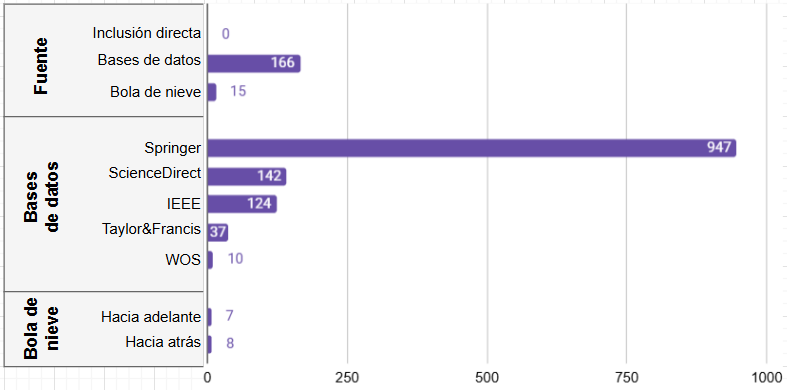
\includegraphics[scale=0.7]{resources/images/Planeacion/procedencia_datos.png}
	\vspace{6pt}
	\caption{SPSs by source and search strategy.}\label{fig:SPSsByProcedence}
\end{figure}

Estos SPS se obtuvieron de bases de datos digitales, identificadas en el SMS mediante diferentes estrategias. La figura~\ref{fig:SPSsByProcedence} muestra el número de estudios recuperados de diversas fuentes y los detalles de las estrategias de búsqueda en bases de datos y de bola de nieve. Independientemente de la fuente, el 91,7\% de los SPS se encontraron mediante la búsqueda en bases de datos, mientras que el 13,16\% restante se identificó mediante la estrategia de bola de nieve.
Independientemente de la estrategia de búsqueda en bases de datos, la figura \ref{fig:SPSsByProcedence} muestra que, de los 99 estudios identificados mediante la búsqueda en bases de datos, el 50,59\% se encontraron en la base de datos ACM, el 24,24\% en ScienceDirect y el 17,17\% en Springer. Entre los 15 SPS identificados mediante bola de nieve, el 40\% se descubrieron mediante bola de nieve hacia atrás y el 60\% mediante bola de nieve hacia adelante.

\begin{figure}[htbp]
	\centering
	\vspace{10pt}
	\includegraphics[scale=0.7]{resources/figures/Venn.png}
	\vspace{6pt}
	\caption{Relationship of SPSs with the research questions.}
	\label{fig:SPSsByRQs}
\end{figure}

Considering the relationships of the SPSs with the RQs, Figure \ref{fig:SPSsByRQs} shows that 100.00\% of the SPSs are related to RQ1, while 24.56\% of the SPSs are simultaneously related to both RQs. Consequently, the remaining 75.44\% are exclusively associated with RQ1. This indicates that no SPS is related solely to RQ2.

\begin{figure}[htbp]
	\centering
	\vspace{10pt}
	\includegraphics[scale=0.7]{resources/figures/SPSsByTopic.jpg}
	\vspace{6pt}
	\caption{Relationship of SPSs with research topics.}
	\label{fig:SPSsByTopics}
\end{figure}

Figure \ref{fig:SPSsByTopics} shows the topics defined during the planning stage for each research question and the number of SPSs inclusively associated with each topic. It is essential to note that one SPS may be linked to multiple topics simultaneously. In this sense, Figure \ref{fig:SPSsByTopics} displays the 12 topics associated with RQ1, where the topic ``Grid Computing'' is the most frequent at 34.21\%. In contrast, the least frequent topics are ``Java'' and ``Checkpointing,'' both at 0.87\%. On the other hand, Figure \ref{fig:SPSsByTopics} also shows the three topics associated with RQ2, where the topic ``Research'' is the most frequent at 16.67\%, while the least frequent is ``industry'' at 2.63\%.

\begin{figure}[htbp]
	\centering
	\vspace{10pt}
	\includegraphics[scale=0.7]{resources/figures/SPSsBYearsAndIndexes.jpg}
	\vspace{6pt}
	\caption{Relationship of SPSs with years of publication and quality indices.}
	\label{fig:SPSsByYearsAndIndexes}
\end{figure}

The search period spans from 1996 to 2024. In this sense, Figure \ref{fig:SPSsByYearsAndIndexes} shows a low number of studies published between 1996 and 2007. In contrast, 2008 recorded an increase compared to 2007, with a total of 6 SPSs. The lowest number of SPSs was in 2009.

According to the SCI index, this SMS presents a relatively regular distribution across all years, with the exception of the period between 2006 and 2015, during which at least one SPS per year met the SCI index. Considering the distribution and the partially regular intervals in which no SPS met this index, this is regarded as an anomaly. Regarding the CVI index, the SMS shows regularity in the number of SPSs per year, particularly from 2017 onwards, except for the period between 2000 and 2008, when no SPS met the CVI index. Considering the IRRQ index, the year 2021 recorded the highest number of studies meeting this criterion, with a total of 5. Furthermore, there is evidence of a fairly consistent trend in the number of SPSs that satisfy this index over the years.

\begin{figure}[htbp]
	\centering
	\vspace{10pt}
	\includegraphics[scale=0.7]{resources/figures/IndexesByTopicAndRQs.jpg}
	\vspace{6pt}
	\caption{Quality indices by topic and research questions.}
	\label{fig:IndexesByTopicAndRQs}
\end{figure}

Figure \ref{fig:IndexesByTopicAndRQs} shows the number of SPSs classified by research question, including their respective topics and considering the quality indices.

In this sense, this study indicates that for RQ1, the topics ``Java'' and ``Checkpointing'' registered the lowest number with 1 SPS each, equivalent to 0.87\% of the 114 SPSs. In contrast, the topic ``Grid Computing'' is the most frequent with 39 SPSs, equivalent to 34.21\% of the 114 SPSs. On the other hand, for RQ2, the most frequent topic is ``Research,'' with 19 SPSs, equivalent to 16.66\% of the 114 SPSs. Conversely, the least frequent topic is ``industry,'' with 3 SPSs, equivalent to 2.63\% of the 114 SPSs.

With respect to the CVI, SCI, and IRRQ indices, we identified the topics ``Java,'' ``Checkpointing,'' and ``industry'' as the categories containing the fewest studies.

\begin{figure}[htbp]
	\centering
	\vspace{10pt}
	\includegraphics[scale=0.7]{resources/figures/SPSsByKeywords.jpg}
	\vspace{6pt}
	\caption{SPSs by keywords.}
	\label{fig:SPSsByKeywords}
\end{figure}

Figure \ref{fig:SPSsByKeywords} shows a cross-analysis between the SPSs, keywords, and synonyms. The synonym ``Work'' enabled the identification of 81 SPSs. Regarding the keyword ``Research,'' it led to the identification of 35 SPSs. In contrast, the keyword ``Universe'' made the smallest contribution, resulting in the identification of no SPSs.

% sub-subsection 4.6.2
\subsubsection{Word Cloud Visualization}

\begin{figure}[htbp]
	\centering
	\vspace{10pt}
	\includegraphics[scale=0.05]{resources/figures/wordcloud.png}
	\vspace{6pt}
	\caption{Word cloud of the keywords.}
	\label{fig:WordCloud}
\end{figure}

Another result obtained from the 114 SPSs of the SMS is the construction of a word cloud. This type of visualization seeks to highlight the most frequent and important words and concepts. Figure \ref{fig:WordCloud} shows the word cloud generated with the tool NubeDePalabras.es, built from the keywords of the SPSs.

Among the most frequent keywords, ``Cloud computing,'' ``Grid computing,'' and ``Distributed computing'' stand out, jointly contributing 18.59\% to the word cloud. The second level of relevance in terms of word cloud corresponds to ``HPC,'' ``High Throughput Computing,'' and ``Scheduling,'' contributing 11.98\%. Finally, a third level includes ``Resource Management,'' ``High Performance Computing,'' and ``Scientific workflow,'' contributing 7.85\%.

It should be emphasized that the calculations were made based on the words included in the cloud. In this case, all words with only one occurrence were excluded, so only words appearing at least twice were considered. This was done to extract the most relevant information. The percentages were then calculated based on the number of occurrences of the words with two or more appearances.


%subsección 4.7
\subsection{Reproducibilidad del método de revisión}\label{sec:reproducibilidad}

Con el objetivo de fomentar la reproducibilidad del método de revisión, se proporcionan dos mecanismos de verificación que permiten a revisores y lectores acceder de forma transparente a la información utilizada en este trabajo, generada mediante la herramienta SMS-Builder~\cite{sms-builder-repo}:

 %Enlace de acceso público a la instancia de SMS-Builder que contiene todos los datos del proceso de revisión sistemática: \url{https://sms-cloud-security.iti.grid.uniquindio.edu.co}. Las credenciales de acceso son \hbox{\textbf{\textit{``admin''}}} tanto para el nombre de usuario como para la contraseña.

 Imagen Docker disponible públicamente que integra toda la documentación necesaria para crear un contenedor con los datos del proceso: \url{https://hub.docker.com/r/parritap/sms-htcondor-universes}.

